\documentclass[10pt]{article}

\usepackage[a4paper,margin=0.78in]{geometry}
\usepackage{amsmath,amssymb,amsthm,mathtools,bm,mathrsfs}
\usepackage{booktabs,tabularx,longtable,microtype,enumitem,multicol,float}
\usepackage{xcolor,tikz}
\usetikzlibrary{arrows.meta,positioning,fit,calc}
\usepackage[colorlinks=true,linkcolor=blue!50!black,
  citecolor=blue!50!black,urlcolor=blue!50!black]{hyperref}
\setlength{\emergencystretch}{2em}

\newtheorem{theorem}{Theorem}
\newtheorem{corollary}[theorem]{Corollary}
\newtheorem{proposition}[theorem]{Proposition}
\newtheorem{lemma}[theorem]{Lemma}
\theoremstyle{definition}
\newtheorem{definition}[theorem]{Definition}
\newtheorem{remark}[theorem]{Remark}

\newcommand{\R}{\mathbb R}
\newcommand{\C}{\mathbb C}
\newcommand{\N}{\mathbb N}
\newcommand{\Z}{\mathbb Z}
\newcommand{\Q}{\mathbb Q}
\newcommand{\T}{\mathbb T}
\newcommand{\ee}{\mathrm e}
\newcommand{\ii}{\mathrm i}
\newcommand{\rank}{\operatorname{rank}}
\newcommand{\Rel}{\mathcal L}
\newcommand{\Hull}{\mathcal K}
\newcommand{\Carrier}{\mathcal C}
\newcommand{\Hwater}{\mathcal H}
\newcommand{\Fid}{\mathcal F}
\newcommand{\dens}{\operatorname{dens}}
\newcommand{\sinc}{\operatorname{sinc}}

\title{\textbf{Persistent phase geometry of quantum recurrence}\\
\large\itshape Four structural laws for loss, spectral constraints, observability, and finite-horizon inference}
\author{GPT 5.6 Sol \and Opus 5 \and Fable 5 \and Michael Haufschild}
\date{27 August 2026}

\begin{document}
\maketitle

\begin{abstract}
Quantum recurrence is usually posed as a question of whether or when a state
returns.  We prove a broader information hierarchy showing that recurrence
has four logically distinct layers.  Loss first selects the persistent
spectral carrier.  On that carrier, convergence of a finite or countable
phase ensemble is equivalent to convergence of every integer-character
action coefficient.  Zero-action characters are exactly the locked spectral
relations, and their rank plus the exposed temporal dimension equals the
full projective phase capacity.  Measurement then forms a strict quotient:
all scalar survival-return experiments determine exactly the spectral
difference measure, while arbitrary observation clocks are themselves
visible only up to time reversal.  By contrast, the complete resolved
replica hierarchy recovers the full projective relation lattice.

This loss of information is strict, not merely formal.  We construct two
explicit uniform nine-level spectra whose scalar survival fidelity agrees at
every time, and hence under every probability law of observation times, but
whose projective relation lattices differ and are separated by a finite
resolved replica detector.  Thus even perfect scalar recurrence data need
not determine completed phase geometry.

The same hierarchy organizes quantitative and many-body results.  It gives
the exact late-return ceiling for finite lossy dynamics, weighted first-hit
bounds, observer-coherence deadlines, arbitrary-spectrum collision laws and
a complete finite-record ambiguity theorem.  Generic static onsite-plus-edge
Hamiltonians on every finite interaction graph attain an exact
component-wise temporal-rank formula; connected nearest-neighbour qudit paths
therefore attain the maximal projective rank.  Their strict completed-time
return density is exponentially small in Hilbert-space dimension and doubly
exponentially small in chain length.  Countable pure-point and bounded
infinite-chain constructions supply corresponding thermodynamic completion
laws.  Circuit-target occupation, recurrent hard epochs, and an explicit
static nearest-neighbour ramp--return--reflection theorem appear as
applications of the same target geometry rather than as a separate account
of recurrence.
\end{abstract}

\noindent\textbf{Public summary.}
Quantum systems can return close to earlier states, but ``the recurrence'' is
not one number.  First ask which part of a system survives loss.  Then ask
which energy phases can move independently.  Next ask which of those phases
a chosen measurement can see.  Only after those questions does it make sense
to ask how often a return occurs or what finite data can predict.

The paper proves that these layers form one exact hierarchy.  It also exposes
a sharp blind spot: two concrete nine-level systems produce identical return
probabilities at every possible time, so no scalar survival experiment can
distinguish them, yet a more resolved multi-copy measurement reveals that
their hidden phase constraints differ.  Perfectly recording one familiar
return signal is therefore not the same as learning the system's full
recurrence structure.

For local many-body systems, spatial simplicity does not imply simple
long-time recurrence.  Generic static nearest-neighbour chains can use every
available relative phase direction, making close returns doubly
exponentially rare with chain length.  The framework also quantifies what
loss erases, what an observer retains, why bounded-time records cannot fix
all future returns, and how circuit complexity must reflect when an exact
return occurs.

\section{One recurrence problem, four structural laws}

The quantum recurrence theorem guarantees arbitrarily accurate returns for
finite closed systems \cite{BocchieriLoinger1957}.  Quantitative work now
bounds recurrence times for broad finite systems
\cite{KotowskiOszmaniec2026,GuptaShort2026}, treats mixed states and
many-body concentration \cite{GimenoSotoca2017,
RiddellPagliaroliAlhambra2023}, and gives exact arithmetic criteria for
Floquet recurrence \cite{AnandEtAl2026}.  Many-body recurrences have been
observed in an isolated quantum gas \cite{RauerEtAl2018}, and coupled-qubit
tests have been proposed \cite{KarimiEtAl2026}.

Yet ``the recurrence time'' is not a sufficient organizing object.  It mixes
four questions with different answers:
\begin{equation}
 \boxed{
 \text{persistent carrier}
 \longrightarrow \text{phase action and relation hull}
 \longrightarrow \text{target metric and observer quotient}
 \longrightarrow \text{finite record}}
 \label{eq:fourquestions-new}
\end{equation}
Loss deletes transient coordinates.  Exact spectral relations cut the ambient
phase torus down to the orbit actually visited.  State weights define how
distance from return is measured, while an observer graph identifies phase
differences that no selected probe can see.  A finite record is finally a
restriction of this already reduced geometry, not a substitute for its
completed arithmetic structure.

This factorization is the paper's universal principle.  Its laws apply to lossy
finite dynamics, arbitrary spectral measures, finite local many-body
Hamiltonians, countable pure-point spectra and specified bounded
infinite-chain models.  They do not claim that all such systems share one
numerical timescale.  They identify which exact object controls each
recurrence question and how that object changes under loss, interaction,
measurement and finite observation.

\subsection{First-principles scope}

Every theorem either starts from an explicitly stated Hamiltonian or
contraction, or proves existence inside an explicitly stated coefficient
class.  States, effects, metrics and target classes are specified.  Deductions
use Born rule, spectral decomposition, unitary evolution,
compact-group characters, exact arithmetic relations, probability measures
and operator-norm circuit approximation.  Randomness, chaos, eigenstate
thermalization and random-matrix statistics are never hidden premises.
Generic conclusions explicitly say generic; exact-model conclusions display
their couplings.

This is first-principles mathematics conditional only on those model axioms.
It is not a microscopic derivation of a laboratory Hamiltonian from a more
fundamental theory of matter.  Experiment therefore tests whether a device
realizes stated carrier, spectrum, coupling graph and measurement map.  It
cannot prove an infinite-time or thermodynamic theorem, but it can falsify
corresponding finite-system predictions.  Section \ref{sec:experiments}
gives concrete protocols and separates these two kinds of claim.

For a finite labelled energy list $E=(E_1,\ldots,E_D)$, global phase is
unobservable, so use the balanced character group
\begin{align}
 P_D&=\left\{k\in\Z^D:\sum_{j=1}^D k_j=0\right\},
 \label{eq:projectivecharacters-new}\\
 \mathcal D_E(k)&=\sum_{j=1}^D k_jE_j,
 \qquad \Rel_E=\ker\mathcal D_E,                       \label{eq:detuning-new}\\
 \tau(E)&=\dim_{\Q}\operatorname{span}_{\Q}
 \{E_j-E_1:2\le j\le D\},                            \label{eq:tau-new}\\
 \rho(E)&=\dim_{\Q}\operatorname{span}_{\Q}\Rel_E.  \label{eq:rho-new}
\end{align}
The relation lattice fixes the projective orbit closure
\begin{equation}
 \Hull_E=\{z\in\T^D/\T:z^k=1\text{ for every }k\in\Rel_E\}. \label{eq:hull-new}
\end{equation}
Its Haar law is the ordinary completed phase ensemble.  For a probability
spectral measure $\mu$, write $\Delta\mu$ for the law of $E-E'$ under two
independent samples.  This difference law is the autocorrelation of the
spectrum and the Fourier transform of the scalar survival fidelity.

\begin{theorem}[Four-law recurrence architecture]
\label{thm:hierarchy}
The following statements hold simultaneously.
\begin{enumerate}[leftmargin=1.65em]
\item Every finite contraction has a unique persistent peripheral carrier;
      all transient contributions vanish and late recurrence occurs entirely
      on this carrier.
\item Along any limiting family of centered uniform observation windows, a
      finite phase law converges weakly if and only if every integer-character
      action coefficient converges.  The same equivalence holds for countable
      spectra using all finite-support characters.
\item For every finite limiting phase law described by zero, finite and
      dephased character actions, zero-action characters are exactly its
      rational constraints and
      \begin{equation}
       \boxed{\text{temporal dimension}+\text{zero-action constraint rank}
       =D-1.}                                         \label{eq:rankconservation}
      \end{equation}
\item Two spectral laws give the same scalar survival-return distribution
      under every probability clock if and only if their difference measures
      $\Delta\mu$ agree.  Dually, two probability clocks give the same scalar
      return distributions for every spectrum if and only if their
      reflection-symmetrized laws agree.
\item Two finite labelled spectra have the same projective relation lattice
      if and only if every resolved replica detector agrees.  This resolved
      hierarchy is strictly more informative than all scalar survival data.
\end{enumerate}
\end{theorem}

Statements two and three are Law II's existence and capacity principles.
They do not assume a
limiting ensemble and then describe it: convergence of all character
coefficients is necessary and sufficient for that ensemble to exist and be
unique.  A phase direction cannot
simultaneously be locked and carry independent temporal motion.  The fourth
and fifth statements begin Law III by identifying two different information levels.  Scalar
survival sees only an autocorrelation; resolved characters recover the
relations themselves.  Weighted targets, observer coherences and finite
records complete Laws III and IV below.

\begin{table}[H]
\centering
\small
\begin{tabularx}{\textwidth}{@{}
  >{\raggedright\arraybackslash}p{0.12\textwidth}
  >{\raggedright\arraybackslash}p{0.24\textwidth}
  >{\raggedright\arraybackslash}X
  >{\raggedright\arraybackslash}X@{}}
\toprule
Law & Exact object & What it determines & Boundary it exposes \\
\midrule
I: carrier & persistent peripheral spectrum & attainable late return ceiling
  and surviving collision law & transient spectral directions \\
II: action & character actions and relation hull & phase-law existence,
  temporal capacity, exact resonances and completed occupation & locked
  relations remove temporal directions \\
III: target & weighted metric and measurement quotient & target cost,
  observer-visible rank, Born deadlines and circuit-target occupation &
  scalar data discard labelled relations and clock orientation \\
IV: record & finite-horizon record class & certified finite-time agreement &
  completed recurrence geometry without additional global information \\
\bottomrule
\end{tabularx}
\caption{The four laws separate dynamical survival, phase capacity,
measurement information and inference.  Each row acts on output of preceding
row.}
\label{tab:hierarchy}
\end{table}

Strictness already appears in nine levels.  Put
\begin{equation}
 C=(0,1,4),\qquad D=(0,10,30),\qquad
 E^{\pm}_{ij}=C_i\pm D_j,                              \label{eq:homometricpair}
\end{equation}
with uniform weight on the nine labelled pairs.  Their amplitudes factor as
$A_+(t)=A_C(t)A_D(t)$ and
$A_-(t)=A_C(t)\overline{A_D(t)}$, hence
\begin{equation}
 |A_+(t)|^2=|A_-(t)|^2\qquad(t\in\R).                 \label{eq:homometricfidelity}
\end{equation}
This equality persists after sampling by every probability clock.  Yet the
balanced character
\begin{equation}
 k_{0,1}=1,\qquad k_{1,0}=-10,\qquad k_{0,0}=9,
 \qquad k_{ij}=0\text{ otherwise}                    \label{eq:witnesscharacter}
\end{equation}
has detuning $0$ for $E^+$ and $-20$ for $E^-$.  The projective relation
lattices therefore differ, and a finite resolved replica detector separates
them.  Product/reflection pairs are classical homometric constructions in
autocorrelation and phase-retrieval theory
\cite{RosenblattSeymour1982,GrimmBaake2008}; the result here is their exact
placement inside a quantum recurrence hierarchy whose scalar quotient is
maximal and whose resolved hierarchy is complete.  Higher-order
autocorrelation completeness and failure are studied in related settings
\cite{YellottIverson1992,AgulnickBusickWarner2026}.

\begin{figure}[H]
\centering
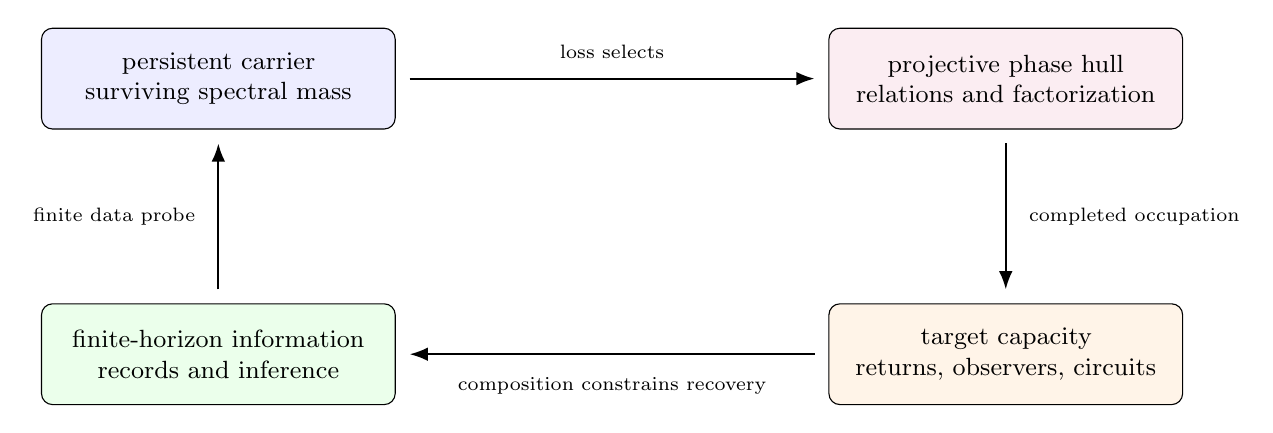
\begin{tikzpicture}[
  font=\small,>=Latex,
  box/.style={draw,rounded corners,align=center,text width=4.0cm,
    minimum height=1.28cm,inner sep=7pt},
  arr/.style={->,thick,shorten >=5pt,shorten <=5pt},
  lab/.style={font=\scriptsize,fill=white,inner sep=2pt}
]
\node[box,fill=blue!7] (p) at (0,3.5)
  {persistent carrier\\surviving spectral mass};
\node[box,fill=purple!7] (h) at (10.0,3.5)
  {projective phase hull\\relations and factorization};
\node[box,fill=orange!9] (c) at (10.0,0)
  {target capacity\\returns, observers, circuits};
\node[box,fill=green!8] (r) at (0,0)
  {finite-horizon information\\records and inference};
\draw[arr] (p) -- node[above=5pt,lab]{loss selects} (h);
\draw[arr] (h) -- node[right=6pt,lab]{completed occupation} (c);
\draw[arr] (c) -- node[below=6pt,lab]{composition constrains recovery} (r);
\draw[arr] (r) -- node[left=6pt,lab]{finite data probe} (p);
\end{tikzpicture}
\caption{\textbf{Persistent phase geometry.}  Exact spectral relations
determine the completed phase hull.  Scalar and resolved observations retain
different quotients of that hull, while finite records need not determine
either completed object.}
\label{fig:architecture}
\end{figure}

Logical dependence matters.  Laws I--IV are structural statements: they say
which mathematical object controls survival, phase motion, visible return and
inference.  Local many-body theorems then ask whether sparse interactions
force Law II's phase hull to be small.  Answer is no for generic
nearest-neighbour paths and yes, with exact ceiling, for fixed-range
commuting l-bits.  First-hit, collision and thermodynamic laws quantify two
sides of this boundary.  Born and circuit results are Law III with concrete
target families, not independent complexity postulates.  Law IV finally
explains why finite records cannot certify completed arithmetic.  One
countable static nearest-neighbour field closes finite-to-infinite loop with
compatible ramps, circuit-hard excursions, recurrence and UHF dynamics.  One
explicit commuting family separately supplies exact recurrence, reflected
descent and failure of pointwise monotonicity.

\section{Law I: loss selects the persistent carrier}

Let $T$ be a contraction on a finite-dimensional complex Hilbert space and
$x$ an initial vector.  Its peripheral spectral projection is denoted
$P_{\mathrm{per}}$ and its persistent mass by
\begin{equation}
 p_{\mathrm{per}}=\|P_{\mathrm{per}}x\|^2.            \label{eq:peripheral-new}
\end{equation}

\begin{theorem}[Persistent-carrier selection]
\label{thm:carrier}
For every finite contraction,
\begin{equation}
 \langle x,T^nx\rangle
 =\sum_{|\lambda|=1}\lambda^n\|P_\lambda x\|^2+r_n,
 \qquad r_n\longrightarrow0.                         \label{eq:persistentdecomp-new}
\end{equation}
The number $p_{\mathrm{per}}$ is the exact asymptotic ceiling of return
amplitude: every sufficiently late amplitude is below
$p_{\mathrm{per}}+\varepsilon$, and values at least
$p_{\mathrm{per}}-\varepsilon$ occur after every prescribed time.  Hence
return amplitude tends to zero exactly when $p_{\mathrm{per}}=0$.  If the
peripheral carrier has at least two levels, every target below
$p_{\mathrm{per}}$ is reached after a finite burn-in and before the explicit
weighted projective deadline of Theorem \ref{thm:water}.
\end{theorem}

The statement covers nonnormal loss as well as unitary dynamics: transient
modes disappear, while the semisimple peripheral packet retains all
recurrence information.

For a probability measure $\mu$ on energy, write
$A_\mu(t)=\int e^{-itE}\,d\mu(E)$ and let
$\Delta\mu$ be the law of $E-E'$ for independent samples from $\mu$.

\begin{theorem}[Arbitrary-spectrum collision hierarchy]
\label{thm:stationary}
For every probability energy spectrum and every $r\in\N$,
\begin{equation}
 \lim_{T\to\infty}\frac1{2T}\int_{-T}^{T}|A_\mu(t)|^{2r}\,dt
 =\bigl((\Delta\mu)^{*r}\bigr)(\{0\}).               \label{eq:wienercollision}
\end{equation}
Every continuous function of survival fidelity has a completed-time mean.
Countable pure-point spectra recur at every positive summable phase-energy
resolution.  A positive exact unit-fidelity return exists exactly when the
visible frequency group is cyclic.  For atomless spectra, projective observer
temporal dimension is the continuum and every fixed positive-fidelity window
has density tending to zero.
\end{theorem}

Pure-point and atomless spectra are extreme cases; mixed spectra remain
covered by collision identity \eqref{eq:wienercollision}.

\section{Law II: phase action converts constraints into temporal capacity}

\subsection{Relations, action and capacity}

For a fixed finite spectrum observed on the centered window $[-T,T]$, the
coefficient of character $k$ is
\begin{equation}
 \frac1{2T}\int_{-T}^{T}e^{-it\mathcal D_E(k)}\,dt
 =\sinc\!\bigl(T\mathcal D_E(k)\bigr).               \label{eq:characteraction}
\end{equation}
It equals one on an exact relation, decays to zero for a fixed nonzero
detuning, and retains a nontrivial finite profile when detuning closes on the
inverse-window scale.  These are the zero, dephased and finite-action regimes
in Theorem \ref{thm:hierarchy}.  Character coefficients determine probability
laws on compact phase groups, which is why their convergence is both
necessary and sufficient rather than only a diagnostic.

\begin{theorem}[Projective phase-capacity law]
\label{thm:phasecapacity}
For every finite real energy list,
\begin{equation}
 \boxed{\tau(E)+\rho(E)=D-1.}                         \label{eq:phasecapacity}
\end{equation}
The temporal dimension of the completed projective phase law is exactly
$\tau(E)$.  A balanced integer character is constant on that law precisely
when it belongs to $\Rel_E$.  At replica order $r$, a resolved detector sees
exactly the locked characters whose positive coefficient mass is at most
$r$.
\end{theorem}

The identity is rank--nullity for the rational detuning map.  It turns an
arithmetic perturbation into an exact conversion law: every relation removed
from a fixed carrier becomes one additional temporal direction.

\begin{theorem}[Arbitrarily weak interaction singularity]
\label{thm:interaction}
Let two nonempty finite spectra have $m+1$ and $n+1$ levels.  For every
$\delta>0$, their tensor-sum Hamiltonian admits a diagonal
operator-Schmidt-rank-one interaction $V=A\otimes B$ with
$\|V\|\le\delta$ such that the perturbed spectrum is maximally projective and
\begin{align}
 \tau(E_A\boxplus E_B)&\le m+n,\\
 \tau(E_A\boxplus E_B+V)&=mn+m+n,                    \label{eq:interactionmult}\\
 \tau(E_A\boxplus E_B+V)-\tau(E_A\boxplus E_B)&\ge mn.
\end{align}
For every bounded observable $O$ and every real $t$,
\begin{equation}
 \|O_V(t)-O_0(t)\|\le2|t|\delta\,\|O\|.              \label{eq:duhamel-main}
\end{equation}
For every positive full-support spectral weight and every replica order, the
perturbed survival-fidelity collision mass equals the unavoidable
permutation floor.
\end{theorem}

Finite-time dynamics is therefore uniformly continuous at every fixed
horizon while completed recurrence geometry can jump by a product-sized
amount.  The singularity is not the universal law itself; it is one sharp
consequence of exact action--constraint conversion.

\subsection{Static local networks}

Let $G=(V,E)$ be any finite simple graph, assign local dimension $q_v\ge2$
to vertex $v$, and allow arbitrary Hermitian onsite terms and arbitrary
Hermitian two-site terms on edges.  For a component $C$, put
$D_C=\prod_{v\in C}q_v$.

\begin{theorem}[Generic temporal rank of a local quantum network]
\label{thm:path}
There is a dense residual full-Lebesgue-measure set of interaction
coefficients such that, simultaneously for every induced subsystem $S$,
\begin{equation}
 \boxed{\tau(H_S)=
 \sum_{C\in\pi_0(G[S])}\left(\prod_{v\in C}q_v-1\right).}
 \label{eq:graphrank-main}
\end{equation}
In particular, if $G$ is connected and
$D=\prod_{v\in V}q_v$, then $\tau(H)=D-1$.
\end{theorem}

The statement includes static open nearest-neighbour qudit paths.  It is
stronger than nondegenerate gaps: it removes every nonconstant balanced
rational relation at once.  Earlier work proved generic nondegenerate gaps
for geometrically local Hamiltonians \cite{Huang2021}; higher no-resonance
conditions are commonly assumed, while chaotic and random-matrix models can
exhibit violations or near violations \cite{RiddellPagliaroli2023}.  Theorem
\ref{thm:path} supplies all orders for
the stated onsite-plus-edge family.

\subsection{Sharp clocks on one static nearest-neighbour path}

Maximal temporal rank becomes a quantitative recurrence statement only after
one specifies a clock.  For $\beta\in\R^d$ and $r>0$, define the first
simultaneous integer-time hit
\begin{equation}
 T_\beta(r)=\min\left\{m\in\N:m\ge1,\
   \max_{1\le j\le d}\lVert m\beta_j\rVert_\Z<r\right\},
 \qquad
 \lVert x\rVert_\Z=\min_{k\in\Z}|x-k|.              \label{eq:local-first-hit}
\end{equation}
For an ordered simple spectrum
$\lambda_1<\cdots<\lambda_D$, use two physically distinct clocks:
\begin{align}
 \beta^{\rm disc}_j&=\frac{\lambda_{j+1}-\lambda_1}{2\pi},
   &&1\le j\le D-1,                                      \label{eq:local-disc-beta}\\
 \beta^{\rm wind}_j&=\frac{\lambda_{j+2}-\lambda_1}
                           {\lambda_2-\lambda_1},
   &&1\le j\le D-2.                                      \label{eq:local-wind-beta}
\end{align}
The first is a stroboscopic laboratory clock.  The second spends the first positive gap
as an internal clock and asks how many windings are needed to align all
remaining gaps.  It is not unrestricted continuous-time first return.

\begin{theorem}[Same-Hamiltonian local saturation and sharp clocks]
\label{thm:local-clock-capstone}
Let $n,q\ge2$, put $D=q^n$, and consider the full real coefficient space of
Hermitian onsite-plus-nearest-neighbour Hamiltonians on the open $n$-site
$q$-level path.  On every nonempty connected open simple-spectrum chart,
one conull set of Hamiltonians simultaneously satisfies:
\begin{enumerate}[label=(\alph*),leftmargin=1.7em]
\item $\Rel_E=\{0\}$ and $\tau(E)=D-1$;
\item
\begin{equation}
 \lim_{r\downarrow0}
 \frac{\log T_{\beta^{\rm disc}}(r)}{\log(1/r)}=D-1,
 \qquad
 \lim_{r\downarrow0}
 \frac{\log T_{\beta^{\rm wind}}(r)}{\log(1/r)}=D-2;
 \label{eq:local-sharp-clocks}
\end{equation}
\item for every strictly positive spectral weight and every replica order,
the collision mass and completed survival-fidelity moment equal the
permutation floor;
\item zero is the only exact anchored projective return time.
\end{enumerate}
One coefficient draw satisfies every clause; the Hamiltonian is not reselected
between rank, clock, collision and exact-return conclusions.
\end{theorem}

Dirichlet approximation supplies exponent upper bounds in
\eqref{eq:local-sharp-clocks}.  Exact path-local spectral escape makes both
gap maps analytically nondegenerate on every simple chart; metric
Diophantine extremality supplies matching lower bounds almost everywhere.
Appendix \ref{app:sharp-local-clocks} gives full argument.  Result is stronger
than nondegenerate gaps and more informative than completed density: it
controls first hits for two stated clocks while preserving same-Hamiltonian
all-order collision conclusions.

\subsection{Exact commuting-local boundary}

The preceding theorem does not say every local model is maximal.  It says
geometric locality alone does not force a deficit.  A commuting l-bit family
exposes additional algebraic restriction exactly.  For $N$ binary modes and
$x\in\{0,1\}^N$, write
\begin{equation}
 E_J(x)=\sum_{S\subseteq\{1,\ldots,N\}}J_S
       \prod_{i\in S}(-1)^{x_i}.                         \label{eq:lbit-energy-main}
\end{equation}

\begin{theorem}[Exact commuting l-bit phase-capacity classification]
\label{thm:lbit-classification-main}
For every real coefficient family,
\begin{equation}
 \boxed{\tau(E_J)=\dim_\Q\operatorname{span}_\Q
   \{J_S:S\ne\varnothing\}},
 \qquad
 \tau(E_J)+\rho(E_J)=2^N-1.                            \label{eq:lbit-rank-main}
\end{equation}
If only one-body coefficients occur, then $\tau(E_J)\le N$.  If every
nonzero support has diameter at most $R$, then
\begin{equation}
 \tau(E_J)\le |\mathcal S_{N,R}|\le N\,2^{R+1},       \label{eq:lbit-range-main}
\end{equation}
where $\mathcal S_{N,R}$ is the family of nonempty allowed supports.  The first
inequality is equality whenever allowed coefficients are rationally
independent; one-body ceiling is attained.  If all nonconstant coefficients
are rationally independent, then $\tau(E_J)=2^N-1$.
\end{theorem}

Walsh orthogonality recovers every $J_S$ from the complete energy packet, so
coefficient span and gap span coincide.  Uniform product state
$|+\rangle^{\otimes N}$ has positive weight on every configuration and sees
full rank; its all-order moments reach permutation floors exactly in the maximal
case.  Contrast is therefore operational.  A fixed-range commuting family
has phase capacity at most linear in $N$, while generic noncommuting
nearest-neighbour path reaches $q^n-1$ despite having only linearly many local
terms.  Parameter-space dimension and rational spectral rank are different
invariants.

\begin{corollary}[Interaction multiplication]
If one edge joins components of dimensions $A$ and $B$, generic temporal
rank changes by
\begin{equation}
 (AB-1)-[(A-1)+(B-1)]=(A-1)(B-1).                     \label{eq:edgegain}
\end{equation}
\end{corollary}

\subsection{Temporal curvature and graph reconstruction}

For distinct vertices $u,v$, define
\begin{equation}
 \kappa(u,v)=\tau(\{u,v\})-\tau(\{u\})-\tau(\{v\}). \label{eq:paircurvature}
\end{equation}

\begin{theorem}[Temporal-curvature reconstruction]
\label{thm:curvature}
On the simultaneous generic set of Theorem \ref{thm:path},
\begin{equation}
 \kappa(u,v)=
 \begin{cases}
 (q_u-1)(q_v-1),&\{u,v\}\in E,\\
 0,&\{u,v\}\notin E,
 \end{cases}
 \qquad
 \{u,v\}\in E\Longleftrightarrow\kappa(u,v)>0.       \label{eq:curvatureedge}
\end{equation}
More generally, for every partition $\Pi$ of $S$,
\begin{equation}
 \tau(S)-\sum_{B\in\Pi}\tau(B)\ge0,                 \label{eq:partitioncurvature}
\end{equation}
with equality exactly when no connected component of $G[S]$ is split across
blocks of $\Pi$.
\end{theorem}

Subsystem decomposition is supplied data.  The theorem reconstructs
interactions relative to that decomposition; it does not derive physical
space from time alone.

\subsection{Exact return density and thermodynamic extinction}

For a Hamiltonian in the generic set of Theorem \ref{thm:path}, with $G$
connected, fix one spectral anchor and define strict chordal return by
\begin{equation}
 \max_{j\ne j_0}|e^{-it(E_j-E_{j_0})}-1|\le\varepsilon.
 \label{eq:anchoredtarget-main}
\end{equation}
For $0<\varepsilon<2$, its completed-time density is
\begin{equation}
 d_D(\varepsilon)=
 \left(\frac{2\arcsin(\varepsilon/2)}{\pi}\right)^{D-1}.
 \label{eq:exactdensity}
\end{equation}
If $D\ge3$, zero is the only exact anchored return time.

\begin{corollary}[Homogeneous-path thermodynamic law]
\label{cor:thermodynamic}
For the generic $n$-site open path of $q\ge2$ levels per site, put
\begin{equation}
 a_\varepsilon=\frac{2\arcsin(\varepsilon/2)}{\pi},
 \qquad I(\varepsilon)=-\log a_\varepsilon.
\end{equation}
After taking completed time at each finite $n$,
\begin{align}
 d_n(\varepsilon)&=a_\varepsilon^{q^n-1},\\
 \frac{-\log d_n(\varepsilon)}{q^n}&\longrightarrow I(\varepsilon),
 \label{eq:thermograph}\\
 \frac1n\log[-\log d_n(\varepsilon)]&\longrightarrow\log q.
 \label{eq:doubleloggraph}
\end{align}
Thus strict completed-time return density is exponentially small in Hilbert
dimension and doubly exponentially small in path length.
\end{corollary}

No infinite-volume evolution or exchange of limits is used in this result.

\begin{theorem}[One-network exhaustion]
\label{thm:exhaustion}
For a countable interaction network exhausted by strictly increasing finite
connected volumes, there is one residual dense set of ambient coefficient
assignments for which every volume simultaneously has
\begin{equation}
 \tau(H_{V_k})=\prod_{v\in V_k}q_v-1\longrightarrow\infty.
 \label{eq:exhaustionrank}
\end{equation}
The same simultaneous event has probability one for every coefficient law
whose finite-volume restriction marginals are absolutely continuous with
respect to Lebesgue measure.
\end{theorem}

This is a finite-volume exhaustion statement, not an infinite-volume rank.

\subsection{All-replica extremality and component factorization}

\begin{theorem}[Nearest-neighbour all-replica floor]
\label{thm:pathcollision}
For every open $n$-site $q$-level path with $n,q\ge2$, a dense residual
full-measure set of onsite-plus-nearest-neighbour Hamiltonians has following
property: for every positive spectral weight and every replica order,
collision mass equals permutation floor, and corresponding long-time
survival-fidelity moment converges to that floor.
\end{theorem}

This is the local interacting contribution.  Exact abstract SFF moments for
rationally independent spectra and related random-walk limits are known
\cite{CamposVenutiOdavicHamma2026}; new content here is simultaneous
all-order spectral premise for a static bounded-degree many-body family.

For a disconnected tensor sum $H=\sum_{r=1}^cH_r$ with mutually transverse,
maximally projective component spectra, let $N_r(X)$ be component-$r$
histogram of an $m$-sample from spectral weights.

\begin{theorem}[Component collision law]
\label{thm:componentcollision}
For every $m\ge1$,
\begin{equation}
 \lim_{T\to\infty}\frac1{2T}\int_{-T}^{T}F(t)^m\,dt
 =\Pr\{N_r(X)=N_r(Y)\ \text{for every }r\}.           \label{eq:histcollision}
\end{equation}
For uniform spectral weights and component dimensions $D_r$,
\begin{equation}
 \lim_{T\to\infty}\frac1{2T}\int_{-T}^{T}
 \left[D^{-1}|\operatorname{Tr}e^{-itH}|^2\right]^m\,dt
 =\prod_{r=1}^c a_{D_r,m},                            \label{eq:sffproduct}
\end{equation}
where
\begin{equation}
 a_{d,m}=d^{-m}\sum_{|k|=m}\binom{m}{k}^{\!2}.        \label{eq:adm}
\end{equation}
For fixed $c$ and $D_r\to\infty$, completed law converges to a product of
$c$ independent unit-mean exponential variables.
\end{theorem}

Joining components replaces equality of marginal histograms by equality of
joint histogram.  Product-sized temporal-rank gain and removal of
factorization-forced replica collisions are two forms of same constraint
conversion.

\subsection{Countable spectra}

\begin{theorem}[Complete saturated recurrence]
\label{thm:countable}
Let a countably infinite spectrum have no nonzero finitely supported balanced
integer relation.  Relative to every anchor, projective relation lattice is
trivial; every future tail of phase orbit is dense in full countable
projective product torus; zero is only exact global return time; and every
strictly positive summable phase-defect probe has lower limit zero, upper
limit its absolute maximum, and crosses every interior level within a
uniformly bounded waiting window from every starting time.

Moreover, every countably infinite real pure-point spectrum admits an
arbitrarily operator-norm-small, domain-preserving, self-adjoint trace-class
diagonal perturbation with all these properties and with unbounded
finite-window temporal rank.  For a product of two countable spectra, one
rank-one separable trace-class interaction direction can be chosen so that
all but a countable set of coupling strengths have complete saturated law.
\end{theorem}

This countable result concerns pure-point diagonal Hamiltonians.  It does not
assert recurrence for continuous spectra or a global return of an infinite
many-body system.

\subsection{A thermodynamic l-bit cascade with Hilbert dynamics}

The countable spectral theorem does not by itself produce an infinite local
Hamiltonian.  A separate construction does.  Let $\Omega=\{\pm1\}^{\N}$ and
let $\chi_S(\sigma)=\prod_{x\in S}\sigma_x$.  There is one explicit real
coefficient field $(J_S)_{S\Subset\N}$ with
\begin{equation}
 \sum_{S\Subset\N}2^{\operatorname{diam}S}|J_S|<\infty.       \label{eq:lbitmass}
\end{equation}
For $0\le g\le1$, define
\begin{equation}
 E_g(\sigma)=\sum_{S\Subset\N}g^{\operatorname{diam}S}J_S\chi_S(\sigma).
 \label{eq:lbitenergy-new}
\end{equation}

\begin{theorem}[Thermodynamic diameter cascade]
\label{thm:lbitcascade}
The series \eqref{eq:lbitenergy-new} converges uniformly on $\Omega$, and
the finite-window energies converge uniformly to $E_g$.  If
$\tau_{n,r}$ denotes temporal dimension of first $n$ sites after retaining
interaction layers of diameter strictly below $r$, then
\begin{equation}
 \tau_{n,r}=\#\{\varnothing\ne S\subseteq\{0,\ldots,n-1\}:
                   \operatorname{diam}S<r\}.                 \label{eq:lbitjetdim}
\end{equation}
Every birth order occurs.  For endpoint support $S_b=\{0,b\}$, its exact
finite-time character reporter at scaled horizon $T=\tau/g^b$, $g\ne0$, is
\begin{equation}
 \mathcal R_b(g,\tau/g^b)
   =\sinc\!\left(\tau\,2^{b+1}J_{S_b}\right).                \label{eq:lbitbirth}
\end{equation}
For every Borel measure $\mu$ on $\Omega$, multiplication by $E_g$ on
$L^2(\Omega,\mu)$ is a bounded self-adjoint Hamiltonian; multiplication by
$e^{-itE_g}$ is a norm-preserving, strongly continuous one-parameter
unitary group.
\end{theorem}

At $g=1$, same field also makes every finite environment $F$ of a local
flip carry maximal temporal rank $2^{|F|}$ while its Heisenberg flip
commutator obeys
\begin{equation}
 \|[\tau_t(X_x),X_y]\psi\|
 \le \min\{2,4K|t|2^{-|x-y|}\}\,\|\psi\|,                 \label{eq:lbitcone}
\end{equation}
where $K$ is weighted mass in \eqref{eq:lbitmass}.  Logarithmic light cones,
spectral line trees and interaction-suppressed revivals are established l-bit
phenomena \cite{KimChandranAbanin2014,NandkishoreGopalakrishnanHuse2014,
VasseurParameswaranMoore2015}.  Contribution here is exact coexistence of
standard infinite-volume Hilbert dynamics, uniform thermodynamic
completion, layer-by-layer phase activation and maximal finite-environment
rational rank in one specified coefficient field.  It is an engineered
diagonal l-bit model, not a theorem for a microscopic random-field chain and
not an infinite-volume global-recurrence claim.

\section{Law III: weights and observers select visible return geometry}

\subsection{Scalar and resolved recurrence}

Let $T$ be sampled from a probability clock $\lambda$, independently of the
spectral law $\mu$, and denote the resulting scalar return law by
\begin{equation}
 \mathscr R(\lambda,\mu)
 =\operatorname{Law}_{T\sim\lambda}\bigl(|A_\mu(T)|^2\bigr). \label{eq:returnlaw}
\end{equation}
Write $\check\lambda(B)=\lambda(-B)$ and
$\lambda^{\rm or}=\tfrac12(\lambda+\check\lambda)$ for the clock with its
orientation forgotten.

\begin{theorem}[Maximal scalar quotients and resolved completeness]
\label{thm:informationquotients}
For probability spectral laws $\mu_1,\mu_2$,
\begin{equation}
 \Delta\mu_1=\Delta\mu_2
 \quad\Longleftrightarrow\quad
 \mathscr R(\lambda,\mu_1)=\mathscr R(\lambda,\mu_2)
 \quad\text{for every probability clock }\lambda.     \label{eq:systemquotient}
\end{equation}
For probability clocks $\lambda_1,\lambda_2$,
\begin{equation}
 \lambda_1^{\rm or}=\lambda_2^{\rm or}
 \quad\Longleftrightarrow\quad
 \mathscr R(\lambda_1,\mu)=\mathscr R(\lambda_2,\mu)
 \quad\text{for every probability spectrum }\mu.     \label{eq:clockquotient}
\end{equation}
For finite labelled spectra, equality of every resolved replica detector is
equivalent to equality of the full projective relation lattice.
\end{theorem}

The word ``maximal'' in this theorem is literal.  The difference measure is
not merely sufficient for scalar survival statistics: no finer invariant of
the spectral law is recoverable from all such statistics, even if the
experimenter may choose every clock.  Likewise, scalar return probability is
even in time, so clock orientation is irretrievably lost.  Resolved replica
characters restore information by retaining labelled phase combinations
before collapsing them to one modulus squared.  Equations
\eqref{eq:homometricpair}--\eqref{eq:witnesscharacter} prove this inclusion is
strict.

\subsection{Weighted recurrence information}

Let $w=(w_1,\ldots,w_D)$ be positive probabilities.  For pivot $k$, define
\begin{align}
 \Hwater_k(w,\eta)&=\min\left\{\frac12\sum_{j\ne k}\log\frac{w_j}{D_j}:
 0<D_j\le w_j,\ \sum_{j\ne k}D_j\le\eta\right\},\\
 \Hwater_{\rm proj}(w,\eta)&=\min_k\Hwater_k(w,\eta). \label{eq:water-new}
\end{align}
Let $T_w(\eta)$ be least integer deadline valid for every compatible phase
packet to return with fidelity at least $(1-\eta)^2$.

\begin{theorem}[Metric-information law]
\label{thm:water}
For $D\ge2$, $0<\eta\le1$,
\begin{align}
 \Hwater_{\rm proj}-\frac\pi4(D-1)-\log(2D)
 &<\log T_w(\eta)                                      \label{eq:deadlinelower-new}\\
 &\le\Hwater_{\rm proj}+(D-1)\log(2\pi\sqrt2).        \label{eq:deadlinelaw-new}
\end{align}
Every compatible phase packet returns after each delay $M$ at some integer
$n$ with $M<n\le(M+1)T_w(\eta)$.
\end{theorem}

Functional is same reverse-water convex program that appears in a parallel
Gaussian rate--distortion calculation
\cite{CoverThomas2006,GrayNeuhoff1998}.  No coding theorem is asserted.

\subsection{Observer coherence}

For a finite family of matrix records, join two energy sectors whenever at
least one weighted observer block contains their coherence.

\begin{theorem}[Observer-coherence law]
\label{thm:observer}
Squared total observer displacement equals a nonnegative weighted edge phase
energy.  It vanishes exactly when phases agree on every connected component
of coherence graph.  If graph has $D$ vertices and $c$ components, visible
projective phase capacity is
\begin{equation}
 \tau_{\rm obs}=D-c.                                  \label{eq:observerrank}
\end{equation}
For every integer resolution $Q$, a positive recurrence time exists no later
than $(Q+1)^{D-c}$, with squared displacement bounded by
\begin{equation}
 4\left(\frac{2\pi}{Q+1}\right)^2
 \sum_{i,j}w^{\rm obs}_{ij}.                          \label{eq:observerdeadline}
\end{equation}
\end{theorem}

Interaction rank and observer rank answer different questions: former counts
phase directions generated by Hamiltonian, latter counts directions visible
to chosen experiment.

\subsection{Born records: escape and return seen by same observer}

State-space recurrence already implies coarse recurrence of bounded
expectation values.  It does not by itself provide an observer-compressed
deadline whose nontrivial exit and later return are both witnessed by same
prescribed record.  Fix an arbitrary finite Hermitian Hamiltonian $H$, a
finite family of density matrices $\rho_a$, quantum effects
$0\le A_a\le I$, and weights $\lambda_a\ge0$.  With
$U(t)=e^{-itH}$, put
\begin{equation}
 B(t)=\sum_a\lambda_a
 \left|\operatorname{tr}\!\left(A_aU(t)\rho_aU(t)^*\right)
             -\operatorname{tr}(A_a\rho_a)\right|.          \label{eq:bornrecord}
\end{equation}

Choose any spectral basis of $H$ and write
$c^a_{ij}=(\rho_a)_{ij}(A_a)_{ji}$ and
$m_{ij}=\sum_a\lambda_a|c^a_{ij}|$.  For a simple graph $G$ on spectral
coordinates, let $c(G)$ be its number of connected components and define
\begin{align}
 M_{\rm sel}(G)&=\sum_{i\sim_Gj}m_{ij},\qquad
 M_{\rm omit}(G)=\sum_{i\ne j,\ i\not\sim_Gj}m_{ij},\nonumber\\
 \mathfrak B(G,Q)&=2M_{\rm omit}(G)+
      \frac{4\pi}{Q+1}M_{\rm sel}(G),                       \label{eq:borndist}\\
 T_*(\varepsilon)&=\min_{\mathfrak B(G,Q)\le\varepsilon}
      (Q+1)^{D-c(G)}.                                       \label{eq:borndeadline}
\end{align}
Here $Q\in\N$; complete graph with sufficiently large $Q$ makes feasible
set nonempty.  Quantity $T_*$ is least clock in this proved
graph--resolution certificate family, not claimed physical first-return
time.

\begin{theorem}[Born-record post-exit recurrence]
\label{thm:bornreturn}
For every data set above, every $\varepsilon>0$ and every guard $g_0>0$,
exactly one of following alternatives is certified:
\begin{enumerate}[leftmargin=1.55em]
\item $B(t)\le\varepsilon$ for every $t\ge0$;
\item there exist $t_{\rm exit}\ge0$ and integer
$1\le n\le T_*(\varepsilon)$ such that
\begin{equation}
 B(t_{\rm exit})>\varepsilon,\qquad
 t_{\rm exit}<n(t_{\rm exit}+g_0)
 \le T_*(\varepsilon)(t_{\rm exit}+g_0),\qquad
 B\!\left(n(t_{\rm exit}+g_0)\right)\le\varepsilon.
 \label{eq:bornreturn}
\end{equation}
\end{enumerate}
No simple spectrum, distinct gaps, noncancellation, randomness, chaos or
genericity assumption is imposed.
\end{theorem}

Recent metric-packing work proves post-exit recurrence for pure states and
identifies expectation-value dynamics as a further direction
\cite{KotowskiOszmaniec2026}; mixed-state recurrence bounds instead control
state-space return \cite{GimenoSotoca2017}.  Theorem \ref{thm:bornreturn}
addresses prescribed finite Born histories, with exit and return in same
record and a deadline compressed by visible coherence graph.  Its novelty
claim is this conjunction, not existence of expectation-value recurrence by
itself.

\subsection{Circuit targets and physical complexity}

Circuit approximation is another observer problem: a gate dictionary selects
a union of target neighbourhoods inside completed phase hull.  This is not a
side application.  It is Law III with an operational target family: phase
motion sets occupation, gate support supplies witnesses, and exact return
constrains entire complexity history.  Next results follow this chain from
generic occupation to one explicit static nearest-neighbour lifecycle.

\subsubsection{Static connected-network Choi occupation}

For a $D$-level Hamiltonian, let $\rho(z)$ be normalized equal-weight Choi
density of phase vector $z$.  Define
\begin{equation}
 B_D(\delta)=D e^{D/2}\left(\sqrt{\pi\delta^2}\right)^{D-1}.
 \label{eq:choicap}
\end{equation}

\begin{theorem}[Generic static-network circuit-target bound]
\label{thm:choicap}
Fix any connected finite interaction graph, local dimensions at least two,
a finite gate alphabet of size $M$, a padded word depth $s$, arbitrary target
density matrices, and $\delta>0$.  On a dense residual full-measure set of
onsite-plus-edge Hamiltonians, upper completed-time occupation of union of
Hilbert--Schmidt $\delta$-balls around all padded targets is at most its
projective Haar volume, and
\begin{equation}
 \overline{\dens}\{t:\rho_H(t)\text{ lies in a padded target ball}\}
 \le M^{s+1}B_D(\delta).                              \label{eq:staticplateau}
\end{equation}
Bound is independent of Hamiltonian eigenbasis.
\end{theorem}

This is a completed-time occupation law, not a claim about monotone growth or
finite-time mixing.

\subsubsection{Static bounded-weight Pauli alternation}

Let $D=2^n$, let $q\ge2$, and let $M_q$ be number of Pauli labels of weight
at most $q$ used by fixed two-query protocol.  For trace-distance tolerance
$\varepsilon>0$, define
\begin{equation}
 \mathcal B_D(\varepsilon)=
 D e^{D/2}
 \left[\sqrt{\pi\,\frac{2(\sqrt2\,\varepsilon)^2}{2}}\right]^{D-1}.
 \label{eq:paulicap}
\end{equation}

\begin{theorem}[Same-Hamiltonian recurrence--hardness alternation]
\label{thm:paulialternation}
Fix a generic real bounded-weight Pauli Hamiltonian, a finite gate alphabet
of size $M$, padded depth $s$, normalized targets containing identity target,
and suppose
\begin{equation}
 M^{s+1}\mathcal B_D(\varepsilon)<1,
 \qquad M_q3^q<D+1.                                   \label{eq:paulibudgets}
\end{equation}
Then one finite $L$ works after every starting time: there is a Choi return
within $\varepsilon$, followed within $L$ by an epoch farther than
$\varepsilon$ from every supplied padded-circuit target, followed within
another $L$ by a second Choi return.  At every real time, including every
hard epoch, product-stabilizer two-query signal is strictly larger than Haar
benchmark $1/(D+1)$.
\end{theorem}

Hamiltonian family contains all Pauli strings of weight at most $q$; it is
$q$-local but not geometrically bounded degree.  Geometric locality is proved
above for temporal rank and all-replica recurrence, not for this
circuit-hardness alternation.

\begin{theorem}[Prime hard polygons]
\label{thm:primepolygon}
Let $p$ be prime, $2r<p$, $0\le\varepsilon<1/2$, and let $Y$ be a finite
dictionary of normalized Choi rays.  If
\begin{equation}
 ((p-1)|Y|)\,r!\,D^{-r}
 <\left(\sqrt{1-4\varepsilon^2}\right)^{2r},           \label{eq:polygonbudget}
\end{equation}
then every maximally projective spectrum has syndetically recurring base
times $\tau$ for which all nonzero vertices
$U_{a\tau}$, $a=1,\ldots,p-1$, avoid every target in $Y$ by more than
$\varepsilon$, while $U_{p\tau}$ returns arbitrarily close to identity.  For
generic bounded-weight Pauli Hamiltonians satisfying second inequality in
\eqref{eq:paulibudgets}, same evolution remains above exact local Haar
benchmark at every time.
\end{theorem}

\subsubsection{One field across growth, hard excursions, recurrence and the thermodynamic limit}

The preceding target laws are finite-dimensional.  We now make size
compatibility literal.  On the countable qubit path, let
\begin{equation}
 H_n(a)=\sum_{j=0}^{n-1}\sum_{\alpha=1}^{3}
   a_{j,\alpha}\sigma_j^\alpha
 +\sum_{j=0}^{n-2}\sum_{\alpha,\beta=1}^{3}
   a_{j,\alpha\beta}\sigma_j^\alpha\sigma_{j+1}^\beta,
 \qquad n\ge3,                                      \label{eq:samefieldH}
\end{equation}
where every $H_n(a)$ is the literal restriction of one coefficient field
$a$.  Let $c$ be the nonscalar Pauli expansion of the infinite nested
$P_{11}$ background in \eqref{eq:nestedH}, and give every onsite or edge
coordinate at position $j$ the open radius
\begin{equation}
 r_j=\frac{10^{-6}}{(j+1)^2}.                         \label{eq:samefieldradius}
\end{equation}
For an $n$-qubit two-qubit circuit $C$, write $\#_2(C)$ for gate count and
put
\begin{equation}
 s_n=\left\lfloor\frac{2^n}{64(n+1)}\right\rfloor,
 \qquad
 \mathcal L_{n,s}=\{zC:|z|=1,\ \#_2(C)\le s\}.       \label{eq:samefieldtarget}
\end{equation}
Gates are arbitrary continuous two-qubit unitaries; no geometric restriction
is imposed on approximating circuit.

\begin{theorem}[Same-field finite-to-thermodynamic recurrence--complexity law]
\label{thm:samefield}
There exists one coefficient field $a$ in \eqref{eq:samefieldH} with following
properties.
\begin{enumerate}[leftmargin=1.7em]
\item It is coordinatewise close to nested background,
      $|a_\ell-c_\ell|<r_j$ for every coordinate $\ell$ at position $j$, and
      $\sum_\ell|a_\ell|<\infty$.  Thus it is static, one-dimensional,
      nearest-neighbour and bounded in total interaction norm.
\item Every finite $H_n(a)$ has simple, maximally projective spectrum.  For
      every $n\ge3$ and $\eta>0$ there is $B_{n,\eta}\ge0$ such that every
      interval $[b,b+B_{n,\eta}]$ contains $t$ and $z\in\C$, $|z|=1$, with
      \begin{equation}
       \|\ee^{-\ii tH_n(a)}-zI\|_{2\to2}<\eta .       \label{eq:samefieldrecurrence}
      \end{equation}
\item On paired prefixes the same field has a quantitative laboratory ramp.
      If $N,K\in\N$, $8\le K$, $8K\le N+2$, $0<\eta\le1/100$, and
      \begin{equation}
       128\pi\eta K\le t<128\pi\eta(K+1),             \label{eq:samefieldrampwindow}
      \end{equation}
      then every circuit approximating
      $\ee^{-\ii tH_{2N+4}(a)}$ within operator error $\eta$ contains at
      least $K$ two-qubit gates.
\item For every sufficiently large $n$, same orbit has perpetual consecutive
      excursions from complete target $\mathcal L_{n,s_n}$.  More precisely,
      there are $W_n>0$ and $G_n,B_n\ge0$ such that for every $b\in\R$ one
      can choose
      \begin{align}
       &u\in[b,b+G_n],\qquad
       t_-\in[u-B_n,u],\qquad
       t_+\in[u+W_n,u+W_n+B_n],                       \label{eq:samefieldtimes}\\
       &t_-<t_+,\qquad W_n\le t_+-t_-,                \notag
      \end{align}
      with both endpoint evolutions within $1/20$ of
      $\mathcal L_{n,s_n}$, whereas for every $t\in(t_-,t_+)$ and every
      $V\in\mathcal L_{n,s_n}$,
      \begin{equation}
       \|\ee^{-\ii tH_n(a)}-V\|_{2\to2}>\frac1{20}.   \label{eq:samefieldhard}
      \end{equation}
      Thus $t_+$ is a literal first re-entry after $t_-$ into closed
      $1/20$ circuit tube, and such excursions occur after every starting
      epoch.
\item The same coefficients define a bounded self-adjoint element
      $H_\infty(a)$ of standard qubit UHF algebra
      \cite{BratteliRobinson1997} and
      \begin{equation}
       U_\infty(t)=\ee^{-\ii tH_\infty(a)},\qquad
       \alpha_t(A)=U_\infty(t)A U_\infty(t)^*          \label{eq:samefieldUHF}
      \end{equation}
      form a norm-continuous unitary group; conjugation defines a point-norm
      continuous one-parameter group of star automorphisms.  For every $T\ge0$ and every
      UHF observable $A$, canonical prefix embeddings satisfy
      \begin{align}
       H_n(a)&\longrightarrow H_\infty(a),             \label{eq:samefieldHconv}\\
       \sup_{|t|\le T}\|\ee^{-\ii tH_n(a)}-U_\infty(t)\|&\longrightarrow0,
                                                               \label{eq:samefieldUconv}\\
       \sup_{|t|\le T}\|\ee^{-\ii tH_n(a)}A\ee^{\ii tH_n(a)}
                    -\alpha_t(A)\|&\longrightarrow0              \label{eq:samefieldAconv}
      \end{align}
\item Put
      \begin{equation}
       S=\|H_\infty(a)\|+2,\qquad
       \delta=\frac1{20S},\qquad
       \beta_n=\left(\frac{2\arcsin(1/10)}{\pi}\right)^{2^n-1},
       \qquad
       \Lambda_n=\frac{\delta}{2\beta_n}-\delta .     \label{eq:desertscale}
      \end{equation}
      Then $\Lambda_n\to\infty$.  For all sufficiently large $n$, after
      every requested epoch $A_0\ge0$ there is $u\ge A_0$ such that
      throughout the whole closed interval $[u,u+\Lambda_n]$,
      \begin{equation}
       \|\ee^{-\ii tH_n(a)}-zI\|_{2\to2}>\frac1{20}
       \qquad(t\in[u,u+\Lambda_n],\ |z|=1).           \label{eq:samefielddesert}
      \end{equation}
      More strongly, after every $A_0$ there are $A_0\le t_-<t_+$ and
      phases $|z_-|=|z_+|=1$ such that
      \begin{align}
       \|\ee^{-\ii t_-H_n(a)}-z_-I\|_{2\to2}&\le\frac1{20},
       &\|\ee^{-\ii t_+H_n(a)}-z_+I\|_{2\to2}&\le\frac1{20},
                                                              \label{eq:samefieldgapends}\\
       \Lambda_n&\le t_+-t_-,
       &\|\ee^{-\ii tH_n(a)}-zI\|_{2\to2}&>\frac1{20}
       \quad(t_-<t<t_+,\ |z|=1).                 \label{eq:samefieldconsecutivegap}
      \end{align}
      Thus $t_-$ and $t_+$ are consecutive visits to closed projective-return
      tube: no further visit lies strictly between them.
      Consequently, although every fixed prefix is syndetically recurrent
      by item 2, no projective-recurrence gap bound at accuracy $1/20$ can
      remain uniform in $n$.  Equivalently, every prescribed return-free
      duration occurs arbitrarily late in all sufficiently large prefixes.
\end{enumerate}
\end{theorem}

This theorem closes four separations left by per-size results.  No
Hamiltonian is redrawn when size changes; ramp, hard excursion, re-entry and
recurrence use literal prefixes of same field; and finite dynamics converge
to standard infinite-volume dynamics.  Finite-volume recurrence survives at
every size, while every volume-independent recurrence clock fails.  Scale
$\Lambda_n$ is not asserted to equal a first-return time measured from zero;
it is a deterministic lower bound on actual arbitrarily late consecutive-return
gaps obtained from exact completed occupation, uniform orbit speed, closedness
of projective-return tube and syndetic recurrence.  Construction is not
translation invariant: absolute summability forces position-dependent decay.  It also
does not assert recurrence or circuit complexity of $U_\infty(t)$ itself.
Those are different infinite-volume questions.

\subsubsection{An exact-return companion: nested local ramp and reflection}

Number qubits consecutively along a path and write
$P_{a,b}=|11\rangle\!\langle11|_{a,b}$.  For $L\ge1$, define
\begin{equation}
 H_L^{\rm nest}=
 \sum_{j=1}^{L}\frac{P_{2j-1,2j}}{j^2}
 +\sum_{j=1}^{L-1}\frac{P_{2j,2j+1}}{(j+1)^4},
 \qquad U_L(t)=\ee^{-\ii tH_L^{\rm nest}}.             \label{eq:nestedH}
\end{equation}
Every nearest-neighbour bond has positive weight, and increasing $L$ leaves
every old term unchanged.  Let $C^{\rm op}_{L,\varepsilon}(t)\in\N\cup\{\infty\}$
be infimum of number of arbitrary two-qubit gates in support-certified
one- and two-qubit circuits $W$ satisfying
$\|W-U_L(t)\|_{2\to2}\le\varepsilon$; one-qubit gates are free.

Lower-bound mechanism is not special to inverse powers or paths.  Let $P$ be
any finite qubit tree, assign real phase $\beta_e$ to each edge, and put
\[
 V_\beta=\exp\!\left(-\ii\sum_{e=\{u,v\}\in E(P)}
   \beta_e |11\rangle\!\langle11|_{uv}\right).
\]

\begin{theorem}[Tree phase-tail obstruction]
\label{thm:phasetail}
Fix $G\in\N$ and $\varepsilon\ge0$.  Suppose that for every deleted set
$N\subseteq E(P)$ with $|N|\le G$,
\begin{equation}
 4\varepsilon<
 \left|\exp\!\left(-\ii\sum_{e\in E(P)\setminus N}|\beta_e|\right)-1\right|.
 \label{eq:phasetail}
\end{equation}
Then every support-certified circuit approximating $V_\beta$ within
operator-norm error $\varepsilon$ uses more than $G$ two-qubit gates.  The
approximating gates may be non-diagonal and may couple arbitrary qubit pairs;
tree restriction applies only to target Hamiltonian.
\end{theorem}

\begin{theorem}[Nested static-local ramp--return law]
\label{thm:nestedramp}
The family \eqref{eq:nestedH} has the following six properties.
\begin{enumerate}[leftmargin=1.7em]
\item For every infinite Boolean configuration $x$, infinite diagonal energy
\begin{equation}
 E_\infty(x)=\sum_{j\ge1}\frac{p_j(x)}{j^2}
 +\sum_{j\ge1}\frac{b_j(x)}{(j+1)^4}                 \label{eq:nestedenergy}
\end{equation}
exists and lies in $[0,3]$.  Its $L$-pair truncation is exactly finite energy
of $H_L^{\rm nest}$, and for $L\ge1$,
\begin{equation}
 0\le E_\infty(x)-E_L(x)\le L^{-1}+L^{-3}             \label{eq:nestedtail}
\end{equation}
uniformly in $x$.  Hence finite energies converge uniformly to one bounded
infinite-chain energy.
\item With $R_L=2\pi(L!)^4$, one has $U_L(R_L)=I$.
\item For every $t$ and $\varepsilon\ge0$,
\begin{equation}
 C^{\rm op}_{L,\varepsilon}(R_L-t)
 =C^{\rm op}_{L,\varepsilon}(t).                     \label{eq:nestedreflection}
\end{equation}
\item If $0<\varepsilon\le1/100$ and
\begin{equation}
 1024\pi\varepsilon\le t\le\frac{\varepsilon L}{2}, \label{eq:nestedwindow}
\end{equation}
then
\begin{equation}
 \left\lfloor\frac{t}{128\pi\varepsilon}\right\rfloor
 \le C^{\rm op}_{L,\varepsilon}(t)
 \le2\left\lceil\frac{2t}{\varepsilon}\right\rceil,\label{eq:nestedramp}
\end{equation}
and same bounds hold at $R_L-t$.
\item For $0<\varepsilon\le1/100$, every $t$ obeying
\eqref{eq:nestedwindow} is a literal positive complexity excursion:
\begin{equation}
 C^{\rm op}_{L,\varepsilon}(0)
 =C^{\rm op}_{L,\varepsilon}(R_L)=0
 <C^{\rm op}_{L,\varepsilon}(t).                  \label{eq:nestedexcursion}
\end{equation}
Consequently complexity is neither nondecreasing nor nonincreasing on the
full return cycle.  Moreover, if $s$ and $t$ both obey
\eqref{eq:nestedwindow} and $1024\pi s\le t$, then
\begin{equation}
 C^{\rm op}_{L,\varepsilon}(s)
 \le C^{\rm op}_{L,\varepsilon}(t).                \label{eq:nestedcoarsemono}
\end{equation}
\item Literal all-pairs monotonicity nevertheless fails inside same window.
For
\begin{equation}
 L=16384,\qquad \varepsilon=2^{-10},\qquad
 s=2\pi-10^{-6},\qquad t=2\pi,                    \label{eq:nestedcountertimes}
\end{equation}
one has
\begin{equation}
 1024\pi\varepsilon\le s<t\le\frac{\varepsilon L}{2},
 \qquad
 C^{\rm op}_{L,\varepsilon}(s)\ge1514,
 \qquad
 C^{\rm op}_{L,\varepsilon}(t)\le1513.            \label{eq:nestedcounter}
\end{equation}
In particular $C^{\rm op}_{L,\varepsilon}(t)<
C^{\rm op}_{L,\varepsilon}(s)$ although $s<t$.
\end{enumerate}
\end{theorem}

This is finite-time circuit hardness for one explicit static bounded-degree
Hamiltonian, not a generic or worst-case ensemble statement.  Ramp means
matching linear envelopes over window \eqref{eq:nestedwindow}.  Equation
\eqref{eq:nestedcoarsemono} excludes scale-separated backtracking, whereas
\eqref{eq:nestedcounter} proves nearby backtracking caused by folded local
phase return.  Couplings decay with position, so theorem
does not claim translation invariance, uniform transport or a complexity
plateau.

\subsubsection{Return forces reflection}

\begin{theorem}[Robust complexity reflection]
\label{thm:reflection}
For autonomous unitary evolution and an inverse-closed gate dictionary, let
$\Delta_R$ be projective Choi return defect at time $R$.  Then
\begin{align}
 C_{\varepsilon+\Delta_R}(U_t)&\le C_\varepsilon(U_{R-t}),\\
 C_{\varepsilon+\Delta_R}(U_{R-t})&\le C_\varepsilon(U_t).
 \label{eq:reflection}
\end{align}
At an exact projective return, robust complexity history is exactly
palindromic: $C_\varepsilon(U_t)=C_\varepsilon(U_{R-t})$.
\end{theorem}

This law constrains decline near recurrence but supplies no first hard time.

\section{Law IV: finite records do not determine completed geometry}

Energy-constrained time series can already exhibit severe extrapolation
limits \cite{ManosWeilenmannNavascues2025}.  The next theorem gives a distinct
static nearest-neighbour ambiguity in which one common earlier record is
compatible with every terminal return probability.

\begin{theorem}[Complete finite-record ambiguity]
\label{thm:ambiguity}
Fix moment order $m$, target time $T>0$, strict earlier horizon
$0\le H<T$, and tolerance $\delta>0$.  There exist one normalized initial
state, one return projector, one common earlier record, and a positive
nearest-neighbour one-particle Hamiltonian $K_p$ for every $p\in[0,1]$ such
that:
\begin{enumerate}[leftmargin=1.55em]
\item all $K_p$ have one common spectrum and are unitarily equivalent;
\item their first $m$ energy moments in fixed initial state agree;
\item their return probabilities are uniformly $\delta$-close to common
      record throughout $[-H,H]$;
\item fixed-protocol return probability at time $T$ is exactly $p$;
\item construction has a particle-number-preserving nearest-neighbour
      free-fermion lift with same complete spectrum in every occupation
      sector.
\end{enumerate}
Every forecaster receiving only common record has terminal absolute error at
least $1/2$ for one compatible system.
\end{theorem}

Perfect-return endpoint forces one zero path coupling in fixed
nearest-neighbour representation; strict subunit probabilities admit a
connected Jacobi representative.  This endpoint rigidity is part of
classification, not an omitted genericity assumption.

There is a complementary all-depth boundary.

\begin{theorem}[Global completion and compact determinacy]
\label{thm:globalcompletion}
No classifier based only on complete polynomial cyclic-local data decides
persistent mean recurrence for all positive-energy spectra with all moments.
Even on a fixed compact positive interval, neither complete perturbative jet
of every bounded continuous spectral observable nor complete all-times
perturbative spectral-form-factor jet universally decides nonperturbative
recurrence phase.  Conversely, if one representative of a complete moment
sequence is supported on a nondegenerate compact interval, then every
probability measure with those moments is identical to it.
\end{theorem}

Finite records, complete local moment data and complete perturbative data are
distinct information regimes.  Compact exact moments cross determinacy
boundary; finite-horizon data do not.

\section{Experimental tests and falsification targets}
\label{sec:experiments}

Experiments do not prove exact arithmetic, infinite-time or thermodynamic
statements.  They test a different proposition: whether a controlled device,
within characterized preparation, Hamiltonian and readout error, realizes a
finite member of the stated mathematical family.  This distinction is especially
important for recurrence because an undetected detuning can become decisive
only beyond the observation window.  Hamiltonian-learning and
randomized-measurement methods provide established routes for model
calibration and nonlinear observable estimation
\cite{WangEtAl2017,ElbenEtAl2023}.  Four direct tests follow from our laws.

\paragraph{Scalar blindness versus resolved recurrence.}
Implement diagonal nine-level Hamiltonians with energies $E^+$ and $E^-$ in
\eqref{eq:homometricpair}, prepare uniform superposition, and measure survival
probability across same time grid.  Law III predicts identical scalar traces
for every time and therefore for every randomized sampling clock.  A second
run measures the resolved character in \eqref{eq:witnesscharacter}, using a
multi-copy interferometric or randomized-measurement realization appropriate
to platform.  That record separates two devices.  Experimental target is not
mere recurrence: it is simultaneous scalar agreement and resolved
disagreement.  A statistically significant scalar mismatch after calibrated
errors would falsify claimed implementation; failure of resolved separation
would falsify either Hamiltonian calibration or measurement map.

\paragraph{Observer-graph quotient.}
For one calibrated finite Hamiltonian, choose two probe families whose
coherence graphs differ by a controlled bridge.  Prepare the same states,
record the same Born observables, and compare return windows.  Theorem
\ref{thm:observer} predicts which phase differences become visible, exact
visible dimension $D-c$, and graph--resolution deadline.  Existing
many-body recurrence experiments already illustrate why recurrence is
observable-relative \cite{RauerEtAl2018}; the present law turns that qualitative
choice into a rank and a finite certificate.  Finite data can test deadline
and zero-set predictions but cannot certify absence of every unmeasured
arithmetic relation.

\paragraph{Local interaction reconstruction and return-density scaling.}
On a programmable qudit chain or small interaction graph, perform calibrated
spectroscopy on induced one- and two-site subsystems.  Candidate temporal
ranks give pair curvature \eqref{eq:paircurvature}; positive curvature should
track programmed edges.  Across increasing path lengths, sample anchored
return condition \eqref{eq:anchoredtarget-main} over expanding time windows
and compare occupation with \eqref{eq:exactdensity}.  This tests finite-volume
predictions and the approach to completed density.  No finite run establishes
rational independence or order of limits in Corollary
\ref{cor:thermodynamic}.

\paragraph{Complexity excursion, exact return and reflection.}
Implement commuting controlled-phase path \eqref{eq:nestedH} for modest $L$,
using independently calibrated bond angles.  Characterize channels near
$0$, a laboratory-window time $t$, reflected time $R_L-t$, and return
$R_L$.  Process measurements test return and reflection; circuit compilation
at fixed operator-norm tolerance searches for matching upper witnesses.
Verified approximation with fewer gates than lower bound in Theorem
\ref{thm:nestedramp} would falsify claimed Hamiltonian or error model.  Failure
to find such circuit does not experimentally prove minimality.  The exact return
period grows rapidly with $L$, so useful near-term tests are small-volume
checks of mechanism rather than direct evidence for thermodynamic limit.

The same-field Theorem \ref{thm:samefield} is not itself a device blueprint.
Its simultaneous coefficient selection is existential, and no finite
experiment realizes UHF limit.  A laboratory test of that stronger theorem
would first require one explicitly calibrated coefficient witness and
finite-size error bounds for chosen observables.  With such witness, process
reconstruction across increasing prefixes could estimate distance to scalar
unitary circle, identify successive entries into closed $1/20$ return tube,
and test whether measured consecutive gaps exceed $\Lambda_n$ within
calibrated uncertainty.  We therefore attach no experimental confirmation
claim to current existential construction or its infinite-volume clause.

These protocols probe different arrows in Figure \ref{fig:architecture}.
None can replace mathematical proof, and no single protocol validates the whole
paper.  Together they distinguish loss, hidden phase constraints,
measurement quotient, local connectivity and return-forced complexity
reflection instead of reporting one undifferentiated recurrence time.

\section{Position relative to current results}

Kronecker--Weyl phase occupation, consequences of rational independence, and
all-order spectral-form-factor moments are established ingredients
\cite{RiddellBertini2024,CamposVenutiOdavicHamma2026}.  Homometric structures
with equal autocorrelation are classical
\cite{RosenblattSeymour1982,GrimmBaake2008}.  The contribution is therefore
not torus averaging or homometry in isolation.  Mathematical center is the
joined persistent-phase factorization: carrier selection, an exact existence
criterion for finite and countable phase laws, action--constraint capacity
conversion, weighted and observer-dependent target geometry, maximal scalar
system and clock quotients, complete resolved tomography, and a sharp
finite-record boundary.  Explicit scalar--resolved separation shows why none
of these layers can be collapsed into one return time.

That hierarchy has following physical realizations and consequences:
\begin{enumerate}[leftmargin=1.6em]
\item loss selects an exact persistent carrier, while arbitrary spectral
      types obey one collision hierarchy and exact approximate-versus-periodic
      recurrence classification;
\item completed temporal dimension has a product-sized discontinuity under
      arbitrarily weak interaction, together with a dimension-free finite-time
      continuity bound and all-replica collision extremality;
\item generic maximal projective rank for every static finite interaction
      graph, simultaneous subsystem graph reconstruction, sharp same-draw
      $D-1$/$D-2$ first-hit clocks on nearest-neighbour paths, exact
      commuting-local compression boundary, and thermodynamic consequences;
\item complete countable-spectrum saturation under arbitrarily weak
      domain-preserving trace-class perturbations and along a separable
      interaction ray outside a countable exceptional set, together with a
      bounded infinite-chain phase cascade;
\item same-record post-exit recurrence for arbitrary finite Hermitian Born
      histories, with least deadline inside exact graph--resolution
      certificate family, and a local finite-record construction compatible
      with every later return probability;
\item static circuit-target occupation and recurrent-hardness laws, plus one
      countable nearest-neighbour coefficient field whose literal prefixes
      share a laboratory complexity floor, near-Hilbert circuit-hard
      excursion--re-entry, syndetic projective recurrence, diverging
      consecutive projective-return gaps and compact-time convergence to one UHF
      dynamics; and one explicit commuting path with
      a two-sided finite-time linear envelope, exact return, exact reflected
      descent, and a certified failure of pointwise monotonicity inside that
      envelope.
\end{enumerate}

Completed-time densities complement rather than replace current first-return
bounds \cite{KotowskiOszmaniec2026,GuptaShort2026}.  Pure- and mixed-state
return theorems do not by themselves supply same-record Born escape and
return with an observer-compressed certificate
\cite{GimenoSotoca2017,KotowskiOszmaniec2026}.  Likewise, higher-order
autocorrelation results address reconstruction from correlation data
\cite{YellottIverson1992,AgulnickBusickWarner2026}; Theorem
\ref{thm:informationquotients} instead identifies exact maximal quantum
survival quotients and proves that resolved recurrence recovers precisely the
projective spectral relation lattice.

Full growth--saturation--recurrence theorems currently concern random circuits
and stochastic Hamiltonian evolution \cite{OszmaniecEtAl2024}.  A static,
time-independent, translation-invariant one-dimensional Hamiltonian can
support exponentially long complexity growth through universal encoded
simulation, but known proof uses computational-complexity assumptions
\cite{BohdanowiczBrandao2017}.  Theorem \ref{thm:samefield} addresses a
different frontier: unconditional existence of one ordinary nearest-neighbour
qubit Pauli field, compatible at every size, with a laboratory lower ramp,
arbitrarily late near-Hilbert circuit-free intervals with consecutive
re-entry, syndetic finite-volume recurrence and a standard UHF thermodynamic
dynamics.  It additionally proves that no projective-recurrence clock can be
uniform in volume: a deterministic return-free scale proportional to inverse
completed return occupation diverges along same literal prefixes and
lower-bounds actual consecutive-return gaps.  This
addresses an existence/lower-gap aspect of current open program of obtaining
tight recurrence bounds for physical local noncommuting Hamiltonians
\cite{KotowskiOszmaniec2026}; it does not give optimal first-return bounds for
all local systems.  Nor does theorem prove exponential-duration complexity
growth, near-maximal saturation, typicality, translation invariance or
infinite-volume recurrence.

These results are also complementary to jump theorems for unitarily invariant
random Hamiltonians \cite{KotowskiOszmaniecHorodecki2025}.  They respect the obstruction that
constant-local time-independent Hamiltonian ensembles need not become Haar
random \cite{CuiEtAl2025}.  A static geometrically local SFF ramp has recently
been proved by a clock embedding \cite{Ippoliti2026}; our completed-time rank
and collision laws address a different regime and do not assert a finite-time
random-matrix ramp.

Unlike random-Hamiltonian jump results, \eqref{eq:nestedcounter} concerns one
explicit deterministic, static, commuting, geometrically nearest-neighbour
Hamiltonian.  It certifies a strict decrease between two specified nearby
times by integer-separated upper and lower bounds.  Thus proposed
``second-law'' behavior of complexity \cite{BrownSusskind2018} cannot be read
as deterministic pointwise monotonicity, even within a window that has
two-sided linear growth envelopes.

Hamiltonian-simulation lower bounds provide important comparison points.
Worst-case one-dimensional piecewise local dynamics require nearly linear
space--time gate count \cite{HaahEtAl2023}; generic commuting two-local
Hamiltonians can require quadratic gate count at short time
\cite{LowEtAl2023}; and recent coefficient-sensitive optimal lower bounds use
local bounded-degree classical hard instances, with time-independent
unit-time constructions and piecewise-constant extensions to later times
\cite{ZlokapaEtAl2026}.  Theorem \ref{thm:nestedramp} is complementary: it
follows one explicit nested static one-dimensional family through a linear
laboratory window, a bounded thermodynamic completion, an exact return and
the reflected complexity history.  It does not claim optimal constants or a
general simulation lower bound.

Completed target occupation is also distinct from Hamiltonian
fast-forwarding and its connection to exponentially precise measurement
\cite{AtiaAharonov2017}, and from explicit transcendence-based examples of
exponential circuit complexity \cite{JiaWolf2023}.

\section{Interpretation and order of limits}

Three distinctions prevent misreading the laws.  First, completed occupation
is a frequency statement, not a first-return estimate: inverse return density
need not equal first hitting time.  Second, thermodynamic density takes
$T\to\infty$ at each fixed finite volume before sending volume to infinity.
The resulting extinction law says that recurrence windows occupy a vanishing
fraction of completed time; it does not say that an infinite-system orbit
returns in operator norm.  The same-field desert theorem adds a deterministic
consequence that density extinction alone does not contain: one
volume-uniform speed scale converts exact finite-volume occupation into
arbitrarily late return-free intervals whose certified length diverges;
closedness and syndeticity then turn these into lower bounds on actual
consecutive-return gaps.  This still is not a first-return distribution, a
first-hit estimate from time zero or an infinite-volume return claim.

Third, physical realization depends on theorem.  Generic graph laws allow
arbitrary onsite and edge terms on the supplied finite graph and do not
assume translation invariance.  The countable results concern pure-point
diagonal spectra.  The l-bit construction supplies a bounded self-adjoint
Hamiltonian, strongly continuous unitary dynamics and uniform finite-volume
completion for one absolutely summable diagonal field.  Theorem
\ref{thm:samefield} instead supplies standard quasi-local $C^*$ dynamics for
one noncommuting nearest-neighbour Pauli field and compact-time convergence of
literal finite prefixes.  Its absolute summability and position-dependent
decay are essential; no translation-invariant or infinite-volume recurrence
claim follows.  The exact-return nested path is static and geometrically
nearest-neighbour with a different, commuting arithmetic structure.  These
hypotheses are part of models, not hidden claims about all local or disordered
systems.

Circuit complexity is included only where recurrence geometry controls a
precisely defined target set.  Completed target occupation does not imply Haar
randomization, and a two-sided linear envelope does not imply monotonicity;
Theorem \ref{thm:nestedramp} proves both scale-separated order and an explicit
nearby backtrack.  Exact return instead enforces the robust reflection law of
Theorem \ref{thm:reflection}.

\section{Synthesis: recurrence as persistent phase geometry}

Four laws answer different versions of the same physical question.  Law I says
whether any recurrent signal remains after loss and gives its exact ceiling.
Law II says what completed motion is possible on the surviving carrier: relations
are locked directions, temporal rank is complementary free capacity, and
local interaction can convert one into the other.  Law III says which portion of
that motion matters for a target or measurement.  Weights set accuracy cost;
observer coherences set visible dimension; scalar survival and resolved
replicas retain provably different information.  Law IV says where finite
data stop: agreement throughout any prescribed horizon need not fix completed
geometry or one later probability.

This organization keeps apparently different results in one theory rather
than one catalogue.  Generic local rank, return-density extinction, countable
completion, Born-record recurrence and circuit complexity all ask how much of
the same phase hull is occupied by a specified target.  Their dimensions differ
because carrier, constraints, weights, observers and record classes differ.
No extra complexity-dynamics postulate is needed to obtain return-forced
reflection, while the explicit local path shows why reflection does not imply
pointwise growth before midpoint.  The same-field theorem supplies missing
finite-to-infinite coherence: early ramp, late hard excursion and recurrence
belong to literal restrictions of one countable Hamiltonian, and those
restrictions converge to one infinite-chain dynamics.  It also resolves
apparent tension between finite recurrence and thermodynamic extinction:
every finite prefix returns with bounded gaps, but necessary gap scale cannot
remain bounded as prefix grows: explicit consecutive gaps diverge.

For interested non-specialists, the central message is concrete.  A system may
look recurrent or nonrecurrent depending on what survived and what is being
measured; even a perfect recording of one return probability can miss hidden
phase organization.  Local interactions do not automatically simplify this
organization, and increasing a chain can make accurate returns occupy an
extraordinarily small share of long times.  For one fixed local field this
rarity is operational: larger prefixes contain arbitrarily long epochs in
which no global phase makes evolution close to identity, even though each
prefix eventually returns again; those epochs sit between certified
consecutive visits to return tube.  Nevertheless exact recurrence,
when engineered, places a global symmetry on complexity history.  The paper turns
these statements into exact laws and marks which parts a finite experiment
can test.

\section{Proof organization}

Appendices give self-contained proofs in order used above.  They begin with
finite contraction selection and arbitrary spectral measures, prove
character completeness, action--constraint conversion, scalar quotient and
resolved relation recovery, and verify strict nine-level witness directly.
They then develop interaction conversion, static-path and arbitrary-graph
genericity, sharp path first-hit clocks, exact commuting l-bit
classification, completed return densities, observer deadlines, Born-record
return, l-bit Hilbert dynamics, circuit-target bounds, countable saturation
and finite-record ambiguity.  Final constructions prove one compatible Pauli
field from finite ramps, recurrent hard excursions and diverging projective
consecutive-return gaps to UHF dynamics,
followed by bounded thermodynamic completion, finite-time circuit ramp, exact
return and reflection for nested static path \eqref{eq:nestedH}.


\appendix
\section{Projective detuning and weak-interaction singularity}

\subsection{Proof of Theorem \ref{thm:phasecapacity}}

For $D=d+1$, scalar-extend the balanced character lattice to the
$d$-dimensional rational space
\[
 P_D^{\Q}=\left\{q\in\Q^D:\sum_jq_j=0\right\}.
\]
The detuning map $\mathcal D_E:P_D^{\Q}\to\R$ is rational-linear.  Its
kernel is the rational span of the balanced integer relation lattice.  Its
range is the rational span of anchored gaps: each generator $E_j-E_1$ is the
image of the balanced character $e_j-e_1$, while every balanced rational
combination reduces to a combination of these anchored gaps.  Rank--nullity
therefore gives
\[
 \dim_{\Q}\operatorname{range}\mathcal D_E+
 \dim_{\Q}\ker\mathcal D_E=D-1.
\]

Pontryagin duality identifies characters fixed by the completed phase law
with integral characters in the detuning kernel.  The operational temporal
dimension is consequently the range rank.  In a replica expansion, a
balanced character of positive mass $h$ first appears at order $h$; phase
cycling annihilates every character of larger mass.  This gives the final
height-filtration statement.

\subsection{Proof of Theorem \ref{thm:interaction}}

Write the product index as
$\{0,\ldots,m\}\times\{0,\ldots,n\}$.  The uncoupled energy is
$E_{ab}=A_a+B_b$.  Its gap space is generated by the $m$ anchored gaps of
$A$ and the $n$ anchored gaps of $B$, so its temporal rank is at most $m+n$.

Write a diagonal rank-one interaction as
$V_{ab}=\alpha_a\beta_b$.  For each nonzero balanced integer character $k$,
its perturbed detuning is a real polynomial in $(\alpha,\beta)$.  This
polynomial is not identically zero: if its uncoupled value vanishes, choose
one pair $(a,b)$ with $k_{ab}\ne0$ and switch on only $\alpha_a$ and
$\beta_b$.  The resulting quadratic coefficient is $k_{ab}$.  The complement
of its zero set is open and dense.  Intersecting these complements over the
countable family of nonzero balanced characters leaves a dense set in every
ball about the origin.  Choose $(\alpha,\beta)$ there with
$\max_{a,b}|\alpha_a\beta_b|\le\delta$.  Then $V=A\otimes B$ is diagonal,
$\|V\|\le\delta$, and the perturbed spectrum is maximally projective.  Its
temporal rank is $(m+1)(n+1)-1=mn+m+n$, proving the rank jump.

For self-adjoint $H,H'$ and $U(t)=e^{-itH}$,
$U'(t)=e^{-itH'}$, Duhamel's formula gives
\[
 U'(t)-U(t)=-i\int_0^t e^{-i(t-s)H'}(H'-H)e^{-isH}\,ds
\]
with reversed orientation for $t<0$, and hence
$\|U'(t)-U(t)\|\le |t|\|H'-H\|$.  Splitting
$U'(t)^*OU'(t)-U(t)^*OU(t)$ into two terms and using unitary invariance gives
$2|t|\|H'-H\|\|O\|$, hence \eqref{eq:duhamel-main}.  Finally, expansion of the $r$th fidelity moment
shows that its non-permutation excess is a sum over unequal multiplicity
vectors of equal total energy.  Maximal projective rank removes every such
balanced equality, leaving exactly the permutation floor.

\section{Arbitrary interaction graphs}

\subsection{Generic component rank}

For a connected two-site graph, the allowed edge term is the full Hermitian
matrix space on the tensor product.  Choose a simple eigenbasis for which
every one-site transition graph is connected and non-bipartite, and choose a
maximally projective eigenvalue list.  The failures of these conditions are
proper real-algebraic sets, so such choices form a nonempty open set inside
the simple-spectrum locus.

Attach a leaf to a tree.  Start from a product extension with layer shifts
chosen to avoid energy collisions.  A small edge perturbation joins the
layer transition graphs.  For every old observer site, the first-order
response of a cross-layer matrix element is a rational function of a layer
gap.  One selected transition contributes a nonzero simple-pole residue;
maximal projective rank prevents cancellation by another oriented gap.
Avoiding the finitely many zeros of these response functions makes every old
transition graph connected while preserving an odd cycle.  The local
matrix algebra at the new leaf supplies its connectivity and odd cycle.

Now suppose a nonconstant balanced rational eigenvalue relation vanished
identically on the enlarged tree-local space.  The second-order response to
the leaf interaction has simple poles indexed by oriented edges of the old
transition graph.  Vanishing residues force relation coefficients to agree
along the categorical product of that graph with the leaf complete graph.
Connectedness and non-bipartiteness make this product connected, so every
coefficient is equal, contradicting nonconstancy.  Thus no balanced relation
polynomial vanishes identically.

Symmetrizing over spectral labels turns each candidate relation into a
polynomial in local Hamiltonian coefficients.  Removing its proper zero set,
the discriminant, and the countable family of rational relations gives a
dense residual full-measure maximal set on every tree.  A spanning tree
embeds into every connected graph, so the same conclusion holds for any
connected graph.

For a disconnected graph, component gap modules add.  Independently scaling
component witnesses avoids the countable set of ratios at which two modules
intersect.  This proves the component formula
\eqref{eq:graphrank-main}.  There are only finitely many induced subsystems;
intersecting their pullbacks supplies one simultaneous generic set.

\subsection{Curvature, density and exhaustion}

On one vertex, temporal rank is $q_v-1$.  On two vertices it is
$q_uq_v-1$ when the edge is present and
$(q_u-1)+(q_v-1)$ otherwise.  Subtraction gives
\eqref{eq:curvatureedge}.  For a partition, refine every connected component
into its connected fragments of dimensions $d_1,\ldots,d_s$.  Its curvature
contribution is
\[
 \prod_{j=1}^s d_j-1-\sum_{j=1}^s(d_j-1),
\]
which is nonnegative for $d_j\ge2$ and vanishes exactly when $s=1$.  Summing
over components proves Theorem \ref{thm:curvature}.

For connected $G$, the anchored phase vector is Haar-equidistributed on
$\T^{D-1}$.  A chordal coordinate lies within $\varepsilon$ of one precisely
on an arc of normalized length
$2\arcsin(\varepsilon/2)/\pi$.  Product Haar measure proves
\eqref{eq:exactdensity}.  Substituting $D=q^n$ and taking logarithms gives
\eqref{eq:thermograph} and \eqref{eq:doubleloggraph}.

For an infinite coefficient product and a finite-volume exhaustion, pull
back each finite-volume generic set along coefficient restriction.  These
maps are continuous open surjections.  The countable intersection of the
residual pullbacks is residual and dense.  Absolute continuity of every
finite marginal makes each bad cylinder null; countable subadditivity gives
the simultaneous probability-one statement.  Since $q_v\ge2$ and volumes
grow strictly, the product dimension minus one tends to infinity.

\section{Replica collisions and component laws}

For positive weights $w_i$, expand the $r$th survival-fidelity moment into
pairs of multiplicity vectors $p,q$ with $|p|=|q|=r$.  A term survives
completed-time averaging exactly when
\[
 \sum_i(p_i-q_i)E_i=0.
\]
Maximal projective rank forces $p=q$, which is precisely the permutation
floor.  Combining this equivalence with the path genericity theorem proves
Theorem \ref{thm:pathcollision}.

For a tensor-sum spectrum, every total energy is a sum of component energies.
Mutual transversality separates a surviving equality component by component;
maximality inside each component then forces equality of the two empirical
histograms.  This proves \eqref{eq:histcollision}.  For uniform weights, the
number of $m$-tuples with histogram $k$ is $\binom{m}{k}$, giving
\eqref{eq:adm} and \eqref{eq:sffproduct}.  At fixed $m$, distinct-label
tuples contribute $m!+O(d^{-1})$, while repeated-label tuples vanish in the
limit.  The factorial moments determine the unit-mean exponential law;
independence of component Haar coordinates gives the product law.

\section{Choi targets and static complexity}

\subsection{Projective Choi tube}

The full $D$-torus splits measure-preservingly into one common phase and a
zero-anchored $(D-1)$-torus.  Equal-weight Choi densities are invariant under
the common phase, so the projective target has exactly the measure of its
full-torus lift.

If a Hilbert--Schmidt target ball is nonempty, choose one captured phase
point.  Every other captured point lies within twice the radius of it.
Pure-state density geometry converts this into a lower bound on normalized
phase overlap.  After rotating the common phase, the inequality
$1-\cos\theta\ge2\theta^2/\pi^2$ puts the relative angles inside a Euclidean
ball.  The standard ball-volume and Gamma bounds give $B_D(\delta)$.  A union
over at most $M^{s+1}$ padded words proves the Haar bound.  Maximal projective
rank transfers it to upper completed-time occupation.  Theorem
\ref{thm:path} supplies that rank on one dense residual full-measure set for
every connected interaction graph, proving Theorem \ref{thm:choicap}.

\subsection{Pauli alternation and hard polygons}

For bounded-weight Pauli coefficients outside the projective relation zero
sets, the Choi energy list is maximally projective.  The strict inequality
in \eqref{eq:paulibudgets} leaves a nonempty open complement to all padded
circuit targets.  Minimality of the projective flow makes both the identity
neighbourhood and this hard complement syndetic.  Applying them successively
gives return--hardness--return within one uniform window length.

The local separator uses the Pauli transfer matrix.  The Hamiltonian
coefficient vector is fixed by autonomous evolution, so the corresponding
local transfer block has Frobenius norm at least one.  Product-stabilizer
twirling weights every output Pauli by $3^{-\operatorname{wt}}$.  Hence the
two-query signal is at least $3^{-q}/M_q$, which exceeds $1/(D+1)$ under the
second inequality of \eqref{eq:paulibudgets}.

For Theorem \ref{thm:primepolygon}, sample a phase vector on the $p$-torsion
grid.  When $2r<p$, congruence of replica multiplicities modulo $p$ is
ordinary equality, so the $2r$th target-overlap moment is at most
$r!D^{-r}$.  Markov's inequality and a union bound over
$(p-1)|Y|$ target--vertex pairs leave one phase vector with every nonzero
multiple hard.  The $p$th multiple is identity.  A nonempty open
neighbourhood of this polygon is visited syndetically by every maximally
projective phase flow.

\section{Countable completion and reflection}

For a countable maximally projective spectrum, every finite restriction has
maximal projective rank.  Its annihilator is therefore trivial, so the orbit
closure is the full product torus.  Removing any bounded initial time does
not change this closure.  Two independent coordinates rule out a nonzero
exact global return.  For a positive summable phase-defect probe, uniform
tail control reduces approximation to finitely many coordinates.  Compact
minimality then gives a bounded hitting window.  Connectedness of the image
and continuity of the probe turn approximate level visits into exact visits
for every interior level.

Absolutely summable diagonal perturbations can be chosen arbitrarily small
and maximally projective on every finite restriction.  They are trace class,
preserve the maximal diagonal domain, and preserve self-adjointness.  A
separable perturbation $u_i v_j$ has the same properties on a product
carrier.  Along its affine coupling ray, each nonzero balanced character can
vanish at at most one coupling unless it annihilates both bare spectrum and
direction.  The chosen direction has no such nonzero character, leaving only
a countable exceptional set.  This proves Theorem \ref{thm:countable}.

Finally, autonomous composition gives
$U_{R-t}=U_RU_t^*$.  Inverting and reversing a word preserves its length in
an inverse-closed dictionary.  Choi-metric unitary invariance and the
triangle inequality add only the return defect $\Delta_R$, proving both
inequalities in \eqref{eq:reflection}.  When $\Delta_R=0$, the two bounds are
inverse inequalities and give exact palindromic symmetry.

\section{Detailed proofs and guide to the results}

These appendices give definitions, exact statements and analytic proofs for
all results summarized in the main text.  They also provide a reader's guide
to the specializations for finite contractions, finite and countable
pure-point spectra, observer families, local spin systems and finite-record
inference.  All arguments are deterministic.  No random-matrix premise,
numerical experiment or unproved nonresonance assumption is used.

\section{Carrier selection and arbitrary spectral type}

\subsection{Finite contractions}

Let $T$ be a contraction on a finite-dimensional complex Hilbert space.
Every eigenvalue satisfies $|\lambda|\le1$.  A Jordan block of size greater
than one on $|\lambda|=1$ would make $\|T^n\|$ grow polynomially, contrary
to $\|T^n\|\le1$.  Hence the peripheral part is semisimple.  Let
$P_\lambda$ be its spectral projections and put
\[
 x_{\rm per}=\sum_{|\lambda|=1}P_\lambda x,
 \qquad M_{\rm per}(T,x)=\sum_{|\lambda|=1}\|P_\lambda x\|^2.
\]

\begin{theorem}[Exact returnability transition]
For every finite contraction and vector,
\[
 \langle x,T^nx\rangle
 =\sum_{|\lambda|=1}\lambda^n\|P_\lambda x\|^2+r_n,
 \qquad r_n\to0.
\]
For every $a<M_{\rm per}(T,x)$ and every burn-in $B$, some $n>B$
satisfies $a\le|\langle x,T^nx\rangle|$.  For every
$a>M_{\rm per}(T,x)$, all sufficiently large $n$ satisfy
$|\langle x,T^nx\rangle|<a$.
\end{theorem}

\begin{proof}
The generalized eigenspaces with $|\lambda|<1$ decay, giving $r_n\to0$.
The peripheral sum is a positive weighted finite phase packet.  Simultaneous
Diophantine approximation returns all its phases arbitrarily close to one
after every delay, so its modulus approaches the sum of its weights,
$M_{\rm per}$, arbitrarily late.  The triangle inequality gives the upper
ceiling; the vanishing transient turns it into an eventual strict bound above
the ceiling.
\end{proof}

If at least two peripheral modes have positive mass, normalize their weights
by $M_{\rm per}$.  Applying the water deadline of Appendix~\ref{app:water} and waiting
until $|r_n|$ is below half the target slack gives an explicit post-burn-in
return below every strict ceiling target.  The same decomposition and
threshold hold termwise for every finite convex mixture of contractions.

\subsection{Stationary spectral measures and collision hierarchy}

For a probability measure $\mu$ on $\R$, let
$\widehat\mu(t)=\int\ee^{\ii tE}\,d\mu(E)$ and let
$\check\mu(A)=\mu(-A)$.  Its difference measure is
$\nu=\mu*\check\mu$, so
$|\widehat\mu(t)|^2=\widehat\nu(t)$.
Write $G_\mu$ for the additive subgroup of $\R$ generated by
$\{E-E':E,E'\in\operatorname{supp}\mu\}$; this is the visible
frequency-difference group.

\begin{theorem}[Stationary spectral return law]
For every $r\ge1$,
\[
 \lim_{T\to\infty}\frac1T\int_0^T
   |\widehat\mu(t)|^{2r}\,dt
 =\nu^{*r}(\{0\}).
\]
Every continuous statistic of $|\widehat\mu(t)|^2\in[0,1]$ has a
long-time mean.  At $r=1$, the mean is
$\sum_E\mu(\{E\})^2$.  Thus the stationary recurrent fidelity is exactly
the point-spectrum collision mass.
\end{theorem}

\begin{proof}
Expand the (2r)-fold product as the Fourier transform of $\nu^{*r}$.
Ces\`aro averaging sends $\ee^{\ii t\omega}$ to the indicator of
$\omega=0$; bounded convergence gives the formula.  Polynomial
approximation on $[0,1]$ extends convergence from moments to every
continuous statistic.
\end{proof}

\begin{theorem}[Pure-point, cyclic and atomless trichotomy]
\leavevmode
\begin{enumerate}[leftmargin=1.6em]
\item Every nonnegative summable countable phase energy
  $\sum_j a_j|\ee^{\ii t\omega_j}-1|^2$ falls below every positive
  resolution at some positive integer time, quantitatively by synchronizing
  a finite head and bounding the summable tail.
\item A probability spectrum has an exact unit-fidelity return at some
  positive time if and only if its visible frequency-difference group is
  cyclic.
\item If $\mu$ is atomless, its projective observer temporal dimension is
  continuum and every fixed positive-fidelity return window has asymptotic
  density zero.
\end{enumerate}
\end{theorem}

The first clause is the countable extension of simultaneous phase recurrence.
The second follows because equality in the triangle inequality forces all
visible phases to coincide.  The third combines atomless difference spectra
with the vanishing Ces\`aro collision mass; the continuum dimension is the
cardinal rank of the atomless phase representation.

\section{Finite projective completion and exact conservation}

Let $I$ be a finite $D$-element carrier and
\[
 P_I=\{k\in\Z^I:\sum_ik_i=0\},\qquad
 D_E(k)=\sum_i k_iE_i,
 \qquad\Rel_E=\ker D_E.
\]
Choose $i_0\in I$ and write
$G_E=\operatorname{span}_{\Q}\{E_i-E_{i_0}\}$.

\begin{theorem}[Projective recurrence completion]
The closure of the relative phase orbit is
\[
 \Hull_E=\Rel_E^\perp
 =\{z\in\T^I/\T:z^k=1\text{ for every }k\in\Rel_E\}.
\]
Haar measure on this hull is the completed phase law.  A balanced character
is almost surely one exactly when it belongs to $\Rel_E$.
\end{theorem}

\begin{proof}
Every relation annihilates the orbit and hence its closure.  Conversely, a
character that annihilates the orbit has real detuning zero, so it lies in
$\Rel_E$.  Equality follows from annihilator duality for compact abelian
groups.
\end{proof}

Tensoring the detuning map with $\Q$ gives an exact sequence
\[
 0\to\ker D_E\to P_I\otimes\Q\xrightarrow{D_E}G_E\to0.
\]
Since $\dim_\Q(P_I\otimes\Q)=D-1$, rank--nullity proves
\[
 \tau(E)+\rho(E)=D-1.
\]
The dimension of $\Hull_E$ is $\tau(E)$.

\subsection{Replica height and phase-grid readout}

Write $k=k^+-k^-$ with disjoint nonnegative parts.  Balancedness gives
$|k^+|_1=|k^-|_1=:h(k)$.  Expanding the $r$th fidelity replica shows that
the character $k$ has positive coefficient exactly when $h(k)\le r$.
Therefore its first possible replica order is $h(k)$, and a replica detects
it exactly when $k\in\Rel_E$ and $h(k)\le r$.

Each order-$r$ phase polynomial has coordinate Fourier bandwidth at most
$r$.  The discrete Fourier transform on a $(2r+1)$-point grid in each
cycled coordinate therefore recovers every coefficient exactly.  A smaller
one-coordinate grid aliases two admissible frequencies, proving worst-case
sharpness.  This proves the replica-height law, exact finite-grid
spectroscopy, and its Nyquist boundary.

\section{Coupling walls and conversion}

For countable profiles $E,W$, define the affine detuning
\[
 D_{E+gW}(k)=D_E(k)+gD_W(k).
\]
If $D_W(k)=0$, the character is either protected for every $g$ or never
crosses.  If $D_W(k)\ne0$, it crosses at the single strength
$-D_E(k)/D_W(k)$.  The character group is countable.

\begin{theorem}[Protected-relation intersection law]
There is a countable $C\subset\R$ such that for every $g\notin C$,
\[
 \Rel_{E+gW}=\Rel_E\cap\Rel_W.
\]
Every open interval contains a nonexceptional strength.  At a transverse
wall, the finite-window character reporter equals
$\sinc(TD_{E+gW}(k))$, with the exact inverse-time crossover profile.
\end{theorem}

The finite completed indicator is discontinuous at the wall, whereas the
reporter is continuous at every finite $T$.  Since arbitrarily small
frequency perturbations can have any prescribed rational rank, every
positive finite temporal-rank stratum is dense and the rank map is nowhere
continuous.  Applying Duhamel's identity to normalized observables gives
all-rank finite-horizon indistinguishability.  Intersecting over an allowed
perturbation space proves that robust relations are precisely
$\Rel_E$ intersected with its annihilator.

\subsection{Complete finite conversion}

Let spectra have $m+1$ and $n+1$ levels.  Their uncoupled product has at
least $mn$ rectangle relations.  A separable diagonal interaction can be
chosen, inside every positive operator-norm budget, so that the coupled
$(m+1)(n+1)$-level spectrum is maximally projective.  Consequently
\begin{align*}
 \rho_{\rm coupled}&=0,\\
 \tau_{\rm coupled}-\tau_{\rm uncoupled}&=\rho_{\rm uncoupled}\ge mn.
\end{align*}
Every positive full-support replica collision moment then equals its
unavoidable permutation floor.  The same interaction obeys the all-probe
bound
\[
 \|U_g(t)OU_g(t)^*-U_0(t)OU_0(t)^*\|
 \le2|t|\,\|H_g-H_0\|\,\|O\|.
\]
The maximal set in the finite separable parameter space is dense, residual
and full measure; its complement remains null in every positive-volume
parameter region.  Combining rational independence with torus
equidistribution gives the deterministic strict/full Haar-frequency
sandwich and the exact uniform-target half-dimensional volume exponent.

\subsection{Countable relation hull and weak recurrence ray}

For a countable pure-point carrier, finite characters still form a countable
group.  Its relation lattice equals the annihilator of the compact orbit
hull, and deleting any finite initial time interval leaves the same hull.
Every positive summable probe is continuous on that hull, so its recurrent
range is a compact interval; endpoints occur as limits, every interior value
is hit exactly, and compactness gives uniformly bounded waiting gaps.

For any two countable self-adjoint pure-point generators, one arbitrarily weak
self-adjoint trace-class separable direction can be chosen maximally
projective on every finite restriction.  Outside one countable coupling set,
the affine sum preserves the original maximal domain and self-adjointness,
has every finite temporal rank, has the full countable projective torus as
every future-tail hull, and has no nonzero exact global return.  Nevertheless
every positive summable probe retains complete syndetic recurrence.  The
finite-window all-probe difference remains bounded by
$2|t||g|\|W\|\|O\|$.

\section{Generic recurrence on a static qudit path}

Let $P_n$ be the open path and let $q\ge2$.  Its physical Hilbert space
has dimension $D=q^n$.  Let $\mathcal L_{P_n,q}^0$ be the trace-zero real
subspace spanned by arbitrary Hermitian onsite terms and finite sums of
Hermitian edge tensors.

\subsection{One local witness}

The proof constructs one simple maximally projective Hamiltonian inductively.
For two sites the edge algebra is the full Hermitian algebra.  A generic
eigenbasis makes the endpoint-observable transition graph complete.  Suppose
a chain has maximal projective energy and a connected non-bipartite endpoint
transition graph.  Attach one $q$-level site with separated diagonal
shifts.  Small edge perturbations activate a spanning family of cross-block
endpoint transitions.  For $q\ge3$, the local complete graph contains a
triangle.  For $q=2$, paired first-order cross- and same-layer transitions
create a triangle.  Simplicity, connectivity and non-bipartiteness persist
on an open set.

For an analytic eigenbranch relation
$\sum_{\alpha,r}c_{\alpha,r}\lambda_{\alpha,r}\equiv0$, vary one edge
matrix element and the shift difference $z=a_r-a_s$.  Second-order
perturbation gives
\[
 \sum_{\alpha,\beta}
 \frac{(c_{\alpha,r}-c_{\beta,s})
 |\langle\psi_\alpha,A\psi_\beta\rangle|^2}
 {z+E_\alpha-E_\beta}=0.
\]
Distinct old gaps make the poles distinct.  Their residues force equality
of coefficients along the categorical product of the endpoint graph with
$K_q$.  Connectedness plus an odd cycle makes this product connected, so
all coefficients are equal.  Only the trace relation survives.  Subtracting
the scalar trace part preserves projective maximality and lands in
$\mathcal L_{P_n,q}^0$.

\subsection{Genericity and recurrence consequences}

For every nonconstant balanced rational coefficient vector, multiply its
eigenvalue linear form over all label permutations.  The product is a
symmetric polynomial, hence a polynomial in characteristic coefficients and
therefore in local Hamiltonian parameters.  The witness proves it is not the
zero polynomial.  Its real zero set is null and nowhere dense.  The
discriminant is handled identically.  Removing the countable union over
rational relations yields a dense full-measure $G_\delta$.

\begin{theorem}[Exact path recurrence law]
For every $n,q\ge2$, the maximal set in
$\mathcal L_{P_n,q}^0$ is dense, residual and full Lebesgue measure.  Every
member has no nonzero balanced integer relation and anchored temporal rank
$q^n-1$.  For $0<\varepsilon<2$,
\[
 \lim_{T\to\infty}\frac1T\left|\left\{0\le t\le T:
 \max_{j\ne j_0}|\ee^{-\ii t(E_j-E_{j_0})}-1|<\varepsilon
 \right\}\right|
 =\left(\frac{2\arcsin(\varepsilon/2)}\pi\right)^{q^n-1}.
\]
No nonzero exact projective return exists.
\end{theorem}

\begin{proof}
The preceding algebraic avoidance proves maximality.  Its balanced-relation
definition gives zero kernel; rational rank of the anchored gaps is therefore
$D-1$.  Kronecker--Weyl equidistribution identifies time frequency with
Haar volume.  Each coordinate target arc has normalized length
$2\arcsin(\varepsilon/2)/\pi$, and independence multiplies the $D-1$
factors.  With at least three levels, two independent anchored frequencies
cannot both have a common nonzero exact period.
\end{proof}

\section{Reverse-water target information and deadlines}
\label{app:water}

Let $w_j>0$, $\sum_jw_j=1$, and $0<\eta\le1$.  For pivot $k$,
\[
 \Hwater_k=\min\left\{\frac12\sum_{j\ne k}\log\frac{w_j}{D_j}:
 0<D_j\le w_j,\ \sum_{j\ne k}D_j\le\eta\right\}.
\]
If $\eta\ge1-w_k$, its value is zero.  Otherwise a unique water level
$\lambda_k>0$ satisfies
$\sum_{j\ne k}\min\{w_j,\lambda_k^{-1}\}=\eta$, and
\[
 D_j^*=\min\{w_j,\lambda_k^{-1}\},\qquad
 \Hwater_k=\frac12\sum_{j\ne k}\log_+(\lambda_kw_j).
\]
Convexity and the Karush--Kuhn--Tucker conditions prove global optimality;
compactness after closing zero-cost inactive coordinates gives attainment.
Minimize over $k$ to obtain $\Hwater_{\rm proj}$.

\subsection{Weighted phase variance}

For phases $z_j\in\T$,
\[
 1-\left|\sum_jw_jz_j\right|^2
 =\frac12\sum_{i,j}w_iw_j|z_i-z_j|^2.
\]
This exact variance identity supplies both the product-box inclusion and the
observer interpretation.

\subsection{Target-volume sandwich}

Fix a pivot and require selected phase coordinates to lie in symmetric arcs
with squared chordal errors proportional to $D_j/w_j$.  The variance
identity shows this product box lies inside the fidelity target.  Its Haar
volume is bounded below by
\[
 \left(\frac{\sqrt2}{\pi}\right)^{r-1}
 \exp\{-\Hwater_{\rm proj}\}.
\]
Conversely, resolve the target by a pivot of maximal weighted alignment and
bound it by a quadratic ellipsoid/product envelope.  Summing over $r$
pivots gives
\[
 \mu_w(\eta)\le
 r\exp\left\{\frac\pi4(r-1)-\Hwater_{\rm proj}\right\}.
\]
Taking minus logarithms proves the two-sided target-information law and the
absolute and relative remainder bounds.  The constructive inner box also
proves strict target-volume positivity.

\subsection{Universal and selected-support clocks}

Round each coordinate resolution to an integer
$Q_j=\lceil\pi\sqrt{2w_j/D_j}\rceil$.  The anisotropic pigeonhole principle
applied to the first $\prod Q_j+1$ phase packets gives two in the same box;
their time difference is a positive return.  Minimizing and comparing the
rounded product with the convex objective proves
\[
 \Hwater_{\rm proj}-\frac\pi4(r-1)-\log(2r)
 <\log T_w
 \le\Hwater_{\rm proj}+(r-1)\log(2\pi\sqrt2).
\]
Applying the same argument to the shifted block of times
$M+1,\ldots,(M+1)T_w$ gives a return after every delay $M$.

For a selected set $S$ and discarded tail mass $\tau_S$, the inequality
\[
 2\tau_S+\sum_{j\in S}D_j\le\eta
\]
is sufficient.  Only $S$ enters the rounded product deadline; the tail pays
twice its weight.  This is an exact certificate for the selected set, not a
claim of joint discrete optimality.

For a phase vector $\omega$, multiplication by any integer $n$ preserves
Haar measure.  A union bound over the first $N$ ticks and the pivot-resolved
target envelope proves the finite-horizon Haar hit bound.  The complementary
mass gives an explicit $1-\alpha$ avoidance quantile whenever the budget is
at most $\alpha$.  Correlations between power-map targets preclude an
equality claim.

Independent onsite phases in a particle-number-preserving local XX spin
Hamiltonian give a diagonal single-excitation block.  The state
$\sum_j\sqrt{w_j}|j\rangle$ has return amplitude
$\sum_jw_jz_j$.  Thus the projective target and its Haar volume transfer
exactly to a local spin ensemble.  A binary construction proves that equal
hard effective support at one operational radius can have different water
entropy and hence different deadline bands.

\section{Observer coherence, operational probes and countable extension}

Let $B_a$ be a finite family of observables, let $b_a(i,j)$ denote the
matrix block from energy sector $j$ to sector $i$, and write
$|b_a(i,j)|$ for its Hilbert--Schmidt norm.  For weights
$\lambda_a\ge0$, put
\[
 W_{ij}=\sum_a\lambda_a|b_a(i,j)|^2,
 \qquad
 \mathcal E(z)=\sum_{i,j}W_{ij}|z_i-z_j|^2.
\]
The coherence graph has edge $ij$ exactly when $W_{ij}>0$.

\begin{theorem}[Finite observer capstone]
For Hamiltonian phases $z_i(t)=\ee^{-\ii tE_i}$, total squared observer
displacement equals $\mathcal E(z(t))$.  This quantity is zero if and only
if phases agree on every edge, equivalently on every connected component.
The range rank of the graph coboundary, and hence visible projective phase
capacity, is $r-c$, where $c$ is the number of components.
\end{theorem}

The identity follows by blockwise expansion.  The zero law uses
nonnegativity.  The rank formula follows because the kernel of the graph
coboundary consists of functions constant on components.

Synchronizing a spanning forest yields a recurrence by
$(Q+1)^{r-c}$ ticks with explicit squared-distance error.  Independent hard
frequencies on a rank-$r-c$ graph show that no smaller universal exponent is
possible.  Cauchy--Schwarz controls every Hilbert--Schmidt normalized linear
probe by total displacement.  An operator contraction has Hilbert--Schmidt
energy at most matrix dimension, giving the square-root dimension conversion;
the identity contraction attains the general factor.  A triangle inequality
adds two calibration errors.  If the resulting tick horizon is below the
certified coherent window, the recurrence is a device-feasible theorem.

For countable pure-point blocks, the same phase-energy identity holds exactly
when the nonnegative edge series is summable.  Truncating to a finite head,
synchronizing it and bounding the tail proves quantitative recurrence and the
zero law.  In the Hamiltonian specialization, zero means every positive
nonzero observer block is phase locked.

\subsection{Equal local information, opposite global recurrence}

There exist two explicit full-rank qutrit states with a common spectrum and
positive spectral weights such that their weighted variance, nonzero
Hilbert--Schmidt speed and nonzero symmetric-logarithmic-derivative quantum
Fisher information agree.  For the same tick protocol, the first returns at
every tick.  The second uses an irrational frequency, has an
inverse-resolution lower bound before return and a matching constructive
upper bound.  Therefore these standard local information quantities do not
determine global recurrence arithmetic.

\section{Complete finite-record ambiguity}

Fix $m\in\N$, $T>0$, $0\le H<T$, and $\delta>0$.  Choose an odd
$n>m$ so large that
\[
 2\left(\sin\frac{\pi H}{2T}\right)^n<\delta.
\]
Let $E_j=\pi j/T$ for $j=0,\ldots,n$, and define
\[
 q_j=2^{-n}\binom{n}{j},\qquad
 r_j=q_j(1+(-1)^{n-j}),\qquad
 w_{p,j}=(1-\sqrt p)q_j+\sqrt p\,r_j.
\]

\subsection{Positive mass and generating functions}

The binomial theorem gives $\sum_jq_j=1$.  The alternating binomial sum
gives $\sum_jr_j=1$, and all weights are nonnegative.  Hence every $w_p$
is a probability measure.  Its amplitude is
\[
 A_p(t)=\left(\frac{1+\ee^{\ii\pi t/T}}2\right)^n
 +\sqrt p\left(\frac{\ee^{\ii\pi t/T}-1}2\right)^n.
\]
At $t=T$, $A_p(T)=(-1)^n\sqrt p$, so $P_p(T)=p$.  Moreover
\[
 |A_p(t)-A_0(t)|=\sqrt p
 \left|\sin\frac{\pi t}{2T}\right|^n,
\]
and because both amplitudes have norm at most one,
\[
 |P_p(t)-P_0(t)|\le2|A_p(t)-A_0(t)|.
\]
This proves uniform continuous-window agreement simultaneously for every
$p\in[0,1]$.

\subsection{Shared Hamiltonian and uniform-field realization}

On $\C^{n+1}$, let $K=\operatorname{diag}(E_0,\ldots,E_n)$ and
$|\psi_p\rangle=\sum_j\sqrt{w_{p,j}}|j\rangle$.  One nonnegative
self-adjoint Hamiltonian therefore realizes all probabilities by varying
normalized preparations.

On $n$ qubits, the permutation-invariant uniform field
\[
 H_{\rm u}=\frac\pi T\sum_{a=1}^n|1\rangle\langle1|_a
\]
has symmetric Dicke eigenvectors of energies $E_j$.  The symmetric pure
state with Dicke-shell weights $w_{p,j}$ reproduces the same amplitude and
moments.  Thus one homogeneous noninteracting Hamiltonian gives the complete
closed-interval ambiguity when preparation may vary.

\subsection{Fixed preparation, projector and spectrum}

Fix $\phi=|0\rangle$.  Choose a unitary $U_p\phi=\psi_p$ and put
$K_p=U_p^*KU_p$.  All $K_p$ are nonnegative, self-adjoint and unitarily
equivalent.  Preparation $\phi$, return projector
$|\phi\rangle\langle\phi|$, spectrum and multiplicities are fixed, while
\[
 \langle\phi,\ee^{\ii tK_p}\phi\rangle=A_p(t).
\]

For $k<n$, the finite-difference identity
\[
 \sum_{j=0}^n(-1)^{n-j}{n\choose j}j^k=0
\]
implies that all $w_p$ have the same energy moments.  This proves the fixed
protocol, arbitrary moment and every-future clauses.

\subsection{Nearest-neighbour path and endpoint rigidity}

For $p<1$, all $w_{p,j}$ are positive.  The Krylov vectors
$\psi_p,K\psi_p,\ldots,K^n\psi_p$ are linearly independent by the
Vandermonde determinant.  Gram--Schmidt yields a basis starting at
$\psi_p$, and self-adjointness makes $K$ tridiagonal in that basis.
Strictly positive spectral weights make every forward Jacobi coupling
nonzero.

At $p=1$, only one parity of energy levels is occupied.  Tridiagonalize the
occupied Krylov block and place the unused levels in a diagonal spectator
block.  This gives a tridiagonal representative with one zero interface
coupling.  Conversely, the endpoint of a connected tridiagonal path is
cyclic: the eigenvalue equation propagates a zero endpoint coordinate through
the path.  An unused eigenvector orthogonal to the fixed endpoint therefore
forces at least one zero coupling.  This proves the exact connectedness
dichotomy and the closed-interval nearest-neighbour realization.

\subsection{Occupation and all-sector fermionic lifts}

Every Hermitian tridiagonal one-particle matrix is the single-excitation block
of a Hermitian particle-number-preserving nearest-neighbour occupation
Hamiltonian, with diagonal onsite terms and adjacent hopping terms.  For the
canonical second quantization,
\[
 d\Gamma(K_p)(u_{j_1}\wedge\cdots\wedge u_{j_k})
 =\left(\sum_{\ell=1}^kE_{j_\ell}\right)
  (u_{j_1}\wedge\cdots\wedge u_{j_k}).
\]
The Slater determinants form a basis.  Thus every $p$ has the same complete
subset-sum spectrum in every fermion-number sector, including multiplicity,
while the recurrence ambiguity remains in the one-excitation protocol.

\subsection{Sharp support and forecast error}

On $r$ common distinct nodes, equality of moments of orders
$0,\ldots,r-1$ gives a square Vandermonde system for the weight difference;
its determinant is nonzero.  Hence distinct measures matching the first
$n$ moments require at least $n+1$ nodes.  The binomial/parity pair uses
exactly $n+1$, so the support threshold is sharp.

Any forecaster receives one input compatible with terminal values zero and
one.  For its real output $y$,
$\max\{|y|,|y-1|\}\ge1/2$.  Therefore every forecasting rule has error at
least $1/2$ on one compatible clock.

\section{Global data boundary}

Finite moments are not the only incomplete local data.  There is no
universal classifier of persistent mean recurrence from complete polynomial
local data on positive-energy spectra with all moments.  Likewise, no
classifier based on the complete perturbative jet of every bounded continuous
spectral observable, or of every perturbative spectral-form-factor order,
works uniformly over compact positive-spectrum families.  The separating
families agree to all specified local or perturbative orders while having
opposite global recurrence phases.

Compact support is the exact positive moment boundary used here.  If two
probability measures are carried by one compact interval and have the same
Hamburger moment sequence, polynomial density in the continuous functions on
that interval makes their integrals agree on every continuous function;
Riesz uniqueness gives equality of measures.

\section{Guide to the results}

\begin{longtable}{@{}>{\raggedright\arraybackslash}p{0.36\textwidth}
  >{\raggedright\arraybackslash}p{0.56\textwidth}@{}}
\toprule
Result & Where established \\
\midrule
\endfirsthead
\toprule
Result & Where established \\
\midrule
\endhead
Projective completion; relation hull; $\tau+\rho=D-1$ & Main Law II;
Appendix Sections C and D \\
Singular wall, sinc profile, dense ranks, bounded-horizon indistinguishability
& Main Theorem 3; Appendix Section D \\
Protected affine relation and complete weak separable conversion & Main
Theorem 3; Appendix Sections D.1--D.2 \\
Countable relation hull and infinite separable recurrence ray & Main Law II;
Appendix Section D.3 \\
Replica height, finite-grid readout and Nyquist sharpness & Main Law II;
Appendix Section C.1 \\
Finite contraction threshold and coupled post-burn-in deadline & Main Law I;
Appendix Section B.1 \\
Stationary point-spectrum scaling and collision hierarchy & Main Law I;
Appendix Section B.2 \\
Countable pure-point recurrence, cyclic exact return and atomless boundary &
Main Law I; Appendix Section B.2 \\
Generic static nearest-neighbour qudit maximality and exact return frequency &
Main Theorem 4; Appendix Section E \\
Weighted projective variance and reverse-water global optimizer & Main Law
III; Appendix Sections F and F.1 \\
Product-box lower law, pivot upper law and two-sided target information & Main
Theorem 5; Appendix Section F.2 \\
Universal deadline, post-delay return, selected support and Haar hit quantile
& Main Theorem 5; Appendix Section F.3 \\
Exact onsite local-spin phase transfer and binary hard-support separation &
Main Law III; Appendix Section F.3 \\
Finite observer phase energy, zero set and graph capacity & Main Theorem 6;
Appendix Section G \\
Sharp graph exponent, probe, calibration and device-window bounds & Main
Theorem 6; Appendix Section G \\
Countable observer recurrence and zero law & Main Law III; Appendix Section
G \\
Equal qutrit local information with opposite global recurrence & Main Law
III; Appendix Section G.1 \\
Positive binomial/parity measures and amplitude identities & Main Law IV;
Appendix Section H.1 \\
One Hamiltonian, uniform-field qubit and fixed-protocol isospectral forms &
Main Theorem 7; Appendix Sections H.2--H.3 \\
Krylov path realization, perfect-return block and forced disconnection & Main
Theorem 7; Appendix Section H.4 \\
Occupation embedding and complete all-sector fermionic spectra & Main Theorem
7; Appendix Section H.5 \\
Common moments, exponential hiding and every exact future & Main Theorem 7;
Appendix Sections H.1--H.3 \\
Vandermonde support threshold and one-half forecast lower bound & Main Law IV;
Appendix Section H.6 \\
Complete local/perturbative nonidentifiability and compact moment determinacy &
Main Law IV; Appendix Section I \\
\bottomrule
\end{longtable}


\section*{Author contributions}
All authors contributed to the conception, mathematical development,
analysis, verification and writing of the manuscript.

\begin{thebibliography}{99}

\bibitem{BocchieriLoinger1957}
P. Bocchieri and A. Loinger,
Quantum recurrence theorem,
\emph{Phys. Rev.} \textbf{107}, 337--338 (1957).

\bibitem{CamposVenuti2015}
L. Campos Venuti,
The recurrence time in quantum mechanics,
arXiv:1509.04352 (2015).

\bibitem{KotowskiOszmaniec2026}
M. Kotowski and M. Oszmaniec,
Tight bounds on recurrence time in closed quantum systems,
arXiv preprint 2601.10409, version 3 (2026).

\bibitem{GuptaShort2026}
C. Gupta and A. J. Short,
Recurrence time for finite quantum systems,
\emph{Phys. Rev. A} \textbf{114}, 012208 (2026);
arXiv:2604.14995.

\bibitem{AnandEtAl2026}
A. Anand, D. Valluri, J. Davis and S. Ghose,
Quantum recurrences and the arithmetic of Floquet dynamics,
\emph{Quantum} \textbf{10}, 2074 (2026).

\bibitem{RauerEtAl2018}
B. Rauer \emph{et al.},
Recurrences in an isolated quantum many-body system,
\emph{Science} \textbf{360}, 307--310 (2018).

\bibitem{KarimiEtAl2026}
B. Karimi, X. Wu, A. N. Cleland and J. P. Pekola,
Blueprint for experiments exploring the quantum recurrence theorem on a
coupled multiqubit system,
\emph{Phys. Rev. Research} \textbf{8}, L012062 (2026).

\bibitem{BrownSusskind2018}
A. R. Brown and L. Susskind,
The second law of quantum complexity,
\emph{Phys. Rev. D} \textbf{97}, 086015 (2018);
arXiv:1701.01107.

\bibitem{OszmaniecEtAl2024}
M. Oszmaniec, M. Kotowski, M. Horodecki and N. Hunter-Jones,
Saturation and recurrence of quantum complexity in random local quantum
dynamics,
\emph{Phys. Rev. X} \textbf{14}, 041068 (2024);
arXiv:2205.09734.

\bibitem{CuiEtAl2025}
L. Cui, T. Schuster, L. Mao, H.-Y. Huang and F. Brand\~ao,
Random unitaries from Hamiltonian dynamics,
arXiv:2510.08434 (2025).

\bibitem{BalasubramanianEtAl2020}
V. Balasubramanian, M. DeCross, A. Kar and O. Parrikar,
Quantum complexity of time evolution with chaotic Hamiltonians,
\emph{J. High Energy Phys.} \textbf{01}, 134 (2020);
arXiv:1905.05765.

\bibitem{AtiaAharonov2017}
Y. Atia and D. Aharonov,
Fast-forwarding of Hamiltonians and exponentially precise measurements,
\emph{Nat. Commun.} \textbf{8}, 1572 (2017);
arXiv:1610.09619.

\bibitem{RiddellBertini2024}
J. Riddell and B. Bertini,
Rationally independent free fermions with local hopping,
\emph{Phys. Rev. E} \textbf{110}, 064101 (2024);
arXiv:2404.12100.

\bibitem{Huang2021}
Y. Huang,
Extensive entropy from unitary evolution,
arXiv:2104.02053 (2021).

\bibitem{CamposVenutiOdavicHamma2026}
L. Campos Venuti, M. Odavi\'c and A. Hamma,
Integrability and chaos via fractal analysis of spectral form factors:
Gaussian approximations and exact results,
\emph{Phys. Rev. E} \textbf{113}, 044128 (2026);
arXiv:2505.05199.

\bibitem{NayakSen2007}
A. Nayak and P. Sen,
Invertible quantum operations and perfect encryption of quantum states,
\emph{Quantum Inf. Comput.} \textbf{7}, 103--110 (2007);
arXiv:quant-ph/0605041.

\bibitem{CoverThomas2006}
T. M. Cover and J. A. Thomas,
\emph{Elements of Information Theory}, 2nd ed. (Wiley, 2006).

\bibitem{GrayNeuhoff1998}
R. M. Gray and D. L. Neuhoff,
Quantization,
\emph{IEEE Trans. Inf. Theory} \textbf{44}, 2325--2383 (1998).

\bibitem{ManosWeilenmannNavascues2025}
T. Manos, M. Weilenmann and M. Navascu\'es,
Timed demolition measurements,
arXiv:2507.06912 (2025).

\bibitem{JiaWolf2023}
Y. Jia and M. M. Wolf,
Hay from the haystack: explicit examples of exponential quantum circuit
complexity,
\emph{Commun. Math. Phys.} \textbf{402}, 141--156 (2023).

\bibitem{Ippoliti2026}
M. Ippoliti,
Provable random-matrix spectral ramp in a static, geometrically local
Hamiltonian,
arXiv preprint 2606.30635, version 1 (2026).

\end{thebibliography}


\end{document}
